This chapter is intended to explore the knowledge that is available in the related literature. The chapter begins with defining the concepts and the terminology. Then, the existing knowledge is taken into consideration, to explored the related facts and to develop the background of the study. Based on the knowledge gathered here, the conceptual framework for the research study is formulated and the methodology and the structure of the study is elaborated, towards the latter part of the chapter.

\section{Terminology}

Here, it is attempted to define and clarify the related terminology which there are a few yet, they are important. There are many different terms which are alternatively in use out there hence, it is crucial to clarify each terms, if they are synonymous, related or not.

\subsection{Randomness}\label{lbl_randomness}

Randomness is defined in many different ways, taking many different aspects into consideration. 
\begin{enumerate}
    \item Cambridge English Dictionary defines randomness as 
    \begin{enumerate}
        \item  "\textit{happening, done, or chosen by chance rather than according to a plan}"\cite{web_cambridge_def_rnd}.
        \item "\textit{by chance, or without being chosen intentionally}"\cite{web_cambridge_def_rnd}.
    \end{enumerate}
    \item According to the Oxford English Dictionary, randomness is "\textit{made, done, or happening without method or conscious decision}"\cite{web_oxford_def_rnd}.
\end{enumerate}

As per the second definition provided by the Cambridge dictionary, the phrase \textit{without being chosen intentionally} emphasises the fact that, there should not be some entity, that influences the choice made by the system. Further, the definition given by the Oxford dictionary also emphasises on the fact that \textit{absolute lack of bias} should be a definite characteristic of randomness.

It is also worth noting that randomness is \textit{not a cause, but an attribute}. There are common misconceptions such as "this was caused by random events" or "this is attributable to random variation" and so forth, which are ideally false. \textit{Randomness} is a term which is coined to attribute when the cause(s) of a particular phenomenon is not known, at least yet. 

\subsection{Non-deterministic Behaviour}\label{lbl_nd_behave}

Behaviour of a system are said to be non-deterministic, even if everything that can be known about a system at a given time is known with all available details about the system, it is still not possible to predict the state at a future time. As per the Cambridge dictionary, "\textit{deterministic}" is an adjective, which means "\textit{Relating to the philosophical doctrine that all events, including human action, are ultimately determined by causes regarded as external to the will}"\cite{web_cambridge_def_determin}.

Some of the problems which demonstrate non-deterministic behaviours are modelled and examined in mathematics and computing related applications. According to Robert W. Floyd, a non-deterministic algorithm is "\textit{a conceptual device to simplify the design of backtracking algorithms}"\cite{art_floyd_non_determin}. A non deterministic algorithm that has f(n) levels might not return the same result on different runs. A non deterministic algorithm may never finish due to the potentially infinite size of the fixed height tree. A prime example of a non-deterministic problem is \textit{Prime Factorisation or Integers} i.e. there is no algorithm that demonstrates deterministic behaviour, to derive the prime factors of a given integer. Primality test is an extension of this problem. When both these problems are taken into consideration, even though we can easily predict the behaviour for small inputs, the system becomes unpredictable, as the inputs grow in their magnitude. There is no known deterministic algorithm that would determine if a given number is a prime or not, other than some repetitive and exhaustive methods.

\subsection{Non-deterministic nature of Randomness}

It is quite evident that the above two subsections \ref{lbl_randomness} and \ref{lbl_nd_behave} describes concepts which are going hand-in-hand. In fact, for a system to be random, one should not be able to precisely predict a future state of the system, even if everything is known about the system to the perfect detail. This leads to the fact that \textit{randomness is non-deterministic} i.e. being non-deterministic is an attribute of randomness.

\subsection{Existence of Randomness}

"\textit{Is randomness really there?}" has been a cause of fascination among scientists, philosophers and so forth. Previously we have established the fact that randomness should essentially have absolute lack of bias, which in other words means that there cannot exists variables that one could manipulate or influence, so that the output becomes predictable. This could also be interpreted as randomness is not something that would cause another. Instead, randomness denotes that we are unaware of what causes the particular effect that we are taking into consideration. In other terms, either we are unaware of, or there is no access to variables that determines the effect of the cause in consideration, making those variables \textit{hidden}. If the previous examples such as Brownian motion, chaotic behaviour of double rod pendulum and so forth, this fact applies on those cases as well. In that sense, we could conclude that randomness exists.

Another perspective one could look at this is that as per Feynman suggests, all interactions are actually taking place across all possible paths, without being ruled out by any other criteria. So there is no randomness involved, nevertheless the experimenter does not have access to absolutely all the information that might affect the set of possible routes to an outcome.

\subsection{Attributes of Randomness - Summary}\label{subsec:rand_attr_sum}

Based on the facts which have been discussed up to now regarding defining randomness, the attributes that true randomness should possess could be itemised as below.

\begin{itemize}
    \item \textbf{Unpredictable}
    \item \textbf{Absolute lack of bias} - This is bi-fold
    \begin{itemize}
        \item System should not demonstrate any bias towards a particular state
        \item It should be infeasible for an outside observer to influence and manipulate the system to be bias to a particular state. This is feasible as long as an outside observer lacks in the knowledge of the system. 
    \end{itemize}
    \item \textbf{Absence of patterns}
    \item \textbf{Non deterministic}
\end{itemize}

\subsection{Forms of Randomness}

Randomness exists in a variety of forms. It is generally accepted that, randomness could primarily be sourced by one of the three (03) origins described below.

\begin{sectionlist}
\subsubsection{Environmental Randomness}

This form of randomness exists in the surroundings of a system. Certain phenomenon such as \textit{Brownian Motion} and \textit{Noise} in signal processing are prime examples for this form of randomness. Since these systems are either completely immune to external influences, or even under external influences the system is not considerably deviated from its non-deterministic  state of behaviour, these systems are ideal in terms of the quality of the randomness.

\subsubsection{Randomness based on Initial Conditions}

The behaviour of certain systems tend to demonstrate an extreme sensitivity to the initial conditions. For an instance we could consider \textit{Double-rod Pendulum}. This is a rod which is rigidly hinged from one end, and has another rod hinged to the other end of the first rod. The farthest edge of the system which is free to move, will form a trajectory when the system is given with an external force.

What is so fascinating about this system is that, a subtle variation of the initial conditions would cause the final trajectory to be drastically different from the previous. This behaviour is known as \textit{Chaotic behaviour} in \textit{Chaos Theory}. This system could be used as a source of randomness, as it demonstrates non-deterministic behaviour. Different initial conditions combined with temporal separation, will yield metrics which are non-deterministic. 

\subsubsection{Randomness generated Intrinsically}

Randomness could also be generated intrinsically. This refers to the behaviour of certain algorithms, routines and so forth, which appears to demonstrate non-deterministic behaviour, given that the initial state of the system is concealed. \textit{\acrfull{prng}s} which are in use in most of the modern day applications, are falling under this classification. This form of randomness is much closely reviewed in later chapters, to determine their performance in terms of complexity, volume and quality. 

\end{sectionlist}

\subsection{Random Generators}

Random generators are machines or systems that would generate a specific type of an output that which it is random. A prominent example of a random generator is a \textit{Lottery Ball Selector} which shuffles the fair light weight balls using a high-speed air flow streamed into an enclosed chamber. It will output a type \textbf{Ball} which is said to be random. In most of the cases, the ball being taken out at random is replaced and the process is repeated. This is considered to have the absolute lack of bias, given that balls are fair.

In applications related to computing, this is slightly more complex. According to \acrfull{nist} USA, one could comprehend generating a random bit sequence, as successive flips of an unbiased coin \, with sides labelled as 0 and 1, with each flip having a probability of 0.5 of producing either 0 or 1\cite{rep_nist_sp_80022}. Further it is worth noting that these flips are independent of each other, i.e. previous flip has no influence whatsoever on the next flip. This is outlined in \acrshort{nist}-SP-800-22 as a perfect random bit generator due to the facts that,

\begin{enumerate}
    \item Values are selected independently at each flip.
    \item Probability on each outcome of the sample space is uniformly distributed, i.e. there is \textbf{absolute lack of bias}. 
\end{enumerate}

It is obvious that this model would not be practical in a cryptographic application. Yet, the hypothetical output of this idealised generator serves the purpose of a benchmark to evaluate the quality of Random Number Generators in general.

\subsection{Quality Attributes of Randomness}

Previously we have arrived at a conclusion that randomness is an attribute of a system. We are leveraging that attribute to be used in certain other systems. For this goal to be attained, we mush essentially look for the following quality attributes of randomness. 
\begin{enumerate}
    \item \textbf{\textit{Complexity}}: Complexity of a RNG is a bi folded attribute. On an attacker's perspective, it should be computationally infeasible to determine the next bit. In that sense, it should be above a predetermined threshold, and higher the complexity, better the system would be. On an owner's perspective, the system should be less complex to implement and maintain. With the least possible effort, the owners should be able to implement and utilise the system.
    
    \item \textbf{\textit{Volume}}: Here it focuses on the amount of random data that could be generated within a given unit time duration. Higher the volume, better the generator would be.
    
    \item \textbf{\textit{Performance}}: Under this attribute, there is a multitude of aspects that need to be taken into consideration. These aspects would include computational complexity in terms of time and space, resource usage, security and so forth. This is also closely related to the volume requirements.
\end{enumerate}

\section{True-Random Generators}

One type of sequence generator is a \acrfull{trng}. A \acrshort{trng} is primarily composed of two main modules. Primarily there is an entropy source at its core. This source is usually based on some microscopic phenomenon that generate statistically random "noise" signals which are of low-level. Examples of such are thermal noise of an electric circuit, the photoelectric effect, involving a beam splitter,timing of user processes (e.g. key strokes or mouse movements), quantum effects in a semiconductor and so forth. Even combination of such could be effectively used. Other component is there to eliminate or mitigate the weaknesses and to improve the quality of the random bits. This process is called "\textit{distillation process}". This distillation process is essential to eliminate possible flaws of the entropy source which could result in producing non-random numbers (e.g. very long strings of zeros or ones).

The outputs of a TRNG could be used directly as a random number. Also, could be fed into a \acrshort{prng} as a seed. To be used directly without any further processing or transformations, the output of any TRNG should comply with \textit{Strict Randomness Criteria} as evaluated by statistical tests in order to determine that the physical sources of the TRNG inputs appear random. For example, an entropy source such as electronic noise might sometimes contain a superposition of certain regular and repetitive structures, such as waves or other periodic phenomena, which might appear to be random, yet would fall short during statistical tests.

\subsection{Limitations of TRNGs}

Even though TRGNs are promising, in terms of quality and randomness, there are several different limitations that would yield them far from usability in applied scenarios. Some of these limitations could be identified as follows.

To be used in cryptographic applications, unpredictability of the outputs is a must. However, certain physical sources (e.g. date/time vectors) are quite predictable. Problems as such could be mitigated by combining a variety of outputs of different types of sources to be used as the inputs for a TRNG. However, the resulting outputs from the TRNG might still be deficient when assessed by statistical tests. Apart from that, generation of high-quality random numbers might be too laborious, leaving such production undesirable in cases where a large quantity of random numbers is required. To produce large quantities of random numbers, PRNGs may be preferred over TRNGs.

On the other hand, most of the phenomenon that has been taken into consideration above, are microscopic. Hence, it is computationally expensive in most of the cases to achieve the performance requirements and most of the times fall short in front of volume requirements. Therefore the required quality attributes are not achieved and they would not be suitable for certain applications such as \textit{Monte-Carlo Simulations} and so forth, which would require large volumes of data.

Another major drawback in TRNG is the requirement of additional hardware which might introduce new dimensions of problems including costs, compatibility and compactness. Almost all of the personal computing is rapidly floating towards leaner and more compact form factors. For an instance we could consider a mobile phone. Plugging in a Hardware RNG to such a device could be far from practicality due to various reasons including size, power supply, processing power required, portability and so forth. So, if there is an RNG which targets at \acrfull{pc} devices, these factors should essentially be taken into consideration.

Following is an itemisation of the commonly found TRNGs in modern applications.

\begin{itemize}
    \item Araneus Alea
    \item ComScire
    \item Entropy Key
    \item Fox-IT Fox RandomCard
    \item ID Quantique
    \item Intel 810/815/840/845G chipsets
    \item LETech
    \item QuintessenceLabs
    \item TectroLabs
    \item TRNG98
    \item VIA Padlock engine
    \item Whitewood Entropy Engine
    \item Kidekin TRNG
    \item OneRNG
    \item BitBabbler
    \item ProtegoST
    \item ubld.it TrueRN
    \item Real Random EaaS
\end{itemize}

Detailed and in-depth examination on these generators are left out from this point forth so as to confine the scope of this study.

\section{Pseudo-Random Generators}

The second generator type is a \acrfull{prng}, also known as \acrfull{drbg}\cite{rep_nist_sp_80057} is an algorithm for generating a sequence of numbers whose properties approximate the properties of sequences of random numbers. A PRNG uses one or more inputs and generates multiple “pseudorandom” numbers. Inputs to PRNGs are called seeds. In contexts in which unpredictability is needed, the seed itself must be random and unpredictable. Hence, by default, a PRNG should obtain its seeds from the outputs of an RNG; i.e., a PRNG requires a RNG as a companion.

The outputs of a PRNG are typically a deterministic function of the seed; i.e., all true randomness is confined to seed generation. The deterministic nature of the process leads to the term “pseudorandom.” Since each element of a pseudorandom sequence is reproducible from its seed, only the seed needs to be saved if reproduction or validation of the pseudorandom sequence is required.

A key weakness of PRNGs is repetition and patterns. Almost all the PRNGs would repeat their sequence after some $n$ number of outputs. Lower the value for $n$, more the system is vulnerable and predictable. For the PRNG to be considered \textit{Cryptographically Secure}, the value of $n$ should be higher. This property is inherent to all the PRNGs. This is why a common form of attack of keeping track of the numbers of the PRNG is possible. However, when the value of $n$ becomes extremely large (e.g. a power of two), it would become temporally infeasible to keep track of each number. Hence it would generate outputs with the required robustness.

In practice, the output from most of the common PRNGs demonstrate certain errors that result them in failing statistical pattern-detection tests. These include:

\begin{itemize}
    \item Shorter than expected periods for some seed states (such seed states may be called 'weak' in this context)
    \item Lack of uniformity of distribution for large quantities of generated numbers
    \item Correlation of successive values;
    \item Poor dimensional distribution of the output sequence;
    \item The distances between where certain values occur are distributed differently from those in a random sequence distribution.
\end{itemize}

However, pseudorandom numbers often appear to be more random than random numbers obtained from physical sources. If a pseudorandom sequence is properly constructed, each value in the sequence is produced from the previous value via transformations that appear to introduce additional randomness. A series of such transformations can eliminate statistical auto-correlations between input and output. Thus, the outputs of a PRNG may have better statistical properties and be produced faster than an RNG.

There are many different PRNG algorithms and systems which are in use in the modern day computing applications. Some of these could be enumerated as follows.

\begin{itemize}
    \item Middle-square method (1946)
	\item Lehmer generator (1951)
	\item Linear Congruential Generator (LCG) (1958)
	\item Lagged Fibonacci Generator (LFG) (1958)
	\item Linear Feedback Shift Register(LFSR) (1965)
	\item Wichmann–Hill generator (1982)
	\item Rule 30 (1983)
	\item Inversive Congruential Generator (ICG) (1986)
	\item Park-Miller generator (1988)
	\item ACORN generator (1989)
	\item MIXMAX generator (1991)
	\item Add-with-carry (AWC) (1991)
	\item Subtract-With-Borrow (SWC) (1991)
	\item Maximally periodic reciprocals (1992)
	\item KISS (1993)
	\item Multiply-with-carry(MWC) (1994)
	\item Complementary-Multiply-With-Carry(CMWC) (1997)
	\item Mersenne Twister(MT) (1998)
	\item Xorshift (2003)
	\item Well Equidistributed Long-period Linear(WELL) (2006)
	\item A small noncryptographic PRNG (JSF) (2009)
	\item Advanced Randomization System (ARS) (2011)
	\item Threefry (2011)
	\item Philox (2011)
	\item SplitMix (2014)
	\item Permuted Congruential Generator (PCG) (2014)
	\item Random Cycle Bit Generator (RCB) (2016)
	\item Xoroshiro128+ (2018)
\end{itemize}

Out of these, \acrfull{lfsr} (1965), Mersenne Twister (1998) and its selected varieties and Xoroshiro128+ (2018) are considered in the following subsections for detailed analysis. These choices are justified under the corresponding subsection.

\subsection{Linear Feedback Shift Register}

In the simplest form, a \acrfull{lfsr} is a \textit{Shift Register}, that will derive its next state based on the immediate previous state. Even though this is susceptible to many vulnerabilities and deviations from the standards of true randomness with cryptographic security, this concept has paved way to many different implementations and innovations in PRNGs such as \acrfull{lcg}s.

\subsubsection{Basic Implementation}

The absolute fundamental implementation is based on the most common bit-wise operator XOR. A popular and simple variety of LFSR is Fibonacci LFSR. Here, certain bit positions are predetermined to be affecting the next state. These predetermined positions are called \textit{Taps}. Current bit at each tap is sequentially XORed together, would be the next bit, which will prepended after shifting the whole register by one bit position. This could be graphically depicted as follows.

The same implemented using Python is as follows.

\begin{code}
\begin{minted}[breaklines,tabsize=2]{py}
import numpy as np

class LSFR:
	def __init__(self, seed, l = 16):
		seedBin = format(seed, '0{0}b'.format(l))
		regTmp = [int(e.encode('ascii')) for e in seedBin]

		self.reg = regTmp[(len(regTmp) - l):]

	def next(self):
		l = len(self.reg)
		nb = self.reg[l - 6] ^ self.reg[l - 4] ^ self.reg[l - 3] ^ self.reg[l - 1]
		self.reg = ([nb] + self.reg)[:l]
		return nb
\end{minted}
\caption{Python implementation of Fibonacci LFSR}
\label{lst:py_class_flfsr}
\end{code}

\subsubsection{Performance and Caveats}

Due to the inherently fast nature of the core operations being used, LFSRs are known to be highly performant in terms of the speed of generation, which makes them useful in applications that requires fast generators. Moreover, the resultant bit sequence demonstrates a considerable statistical quality. Yet, it suffers from the major weaknesses enumerated below.

\begin{enumerate}
    \item LFSR generates a deterministic output stream. Given that the present state of the LFSR along with the positions of taps, one could derive the next states easily.
    \item Output streams are reversible; a LFSR with mirrored taps will cycle through the output sequence in reverse order.
\end{enumerate}

\subsection{Mersenne Twister}

\acrfull{mt} is a 623-dimensionally equidistributed uniform pseudorandom number generator. The most commonly used version of the Mersenne Twister algorithm is based on the Mersenne prime $2^{19937}−1$ (hence the name). This is precisely the period of the particular implementation. The algorithm is based on a definition of a $k$-distribution as \textit{a very reasonable definition of randomness}\cite{art_mt_tomacs_urng}. This was chosen mainly due to that fact that this is one of the most commonly adopted random generator in many applications and libraries including but not limited to Microsoft Excel\cite{misc_merald_excel}, MATLAB\cite{web_matworks_randstream}, PHP\cite{web_php_manual_mtrand}, Python\cite{web_python2_manual_prng}\cite{web_python3_manual_prng}, C++ (V.11 and forth)\cite{rep_rand_cpp} and CUDA\cite{web_cuda_rand}. As for the pros and cons, following could be enumerated.

\subsubsection{Pros}

\begin{itemize}
    \item Licensed permissively and royalty-free for all of its variants except CryptMT.
    \item A substantially large interval of $2^{19937} − 1$ (in MT19937 implementation)
    \item Included in many programming languages and libraries.
    \item Passes a variety of statistical tests, including the Diehard tests and most of the TestU01 tests.
    \item $k$-distributed to 32-bit accuracy for every $1 \leq k \leq 623$
    \item Generally faster than other methods. A study indicates that the Mersenne Twister generates 64-bit floating point random numbers approximately twenty times faster than the hardware-implemented, processor-based RdRand instruction set.\cite{art_route_astrophysical_jrn}
\end{itemize}

\subsubsection{Cons}

\begin{itemize}
    \item Relatively large state buffer(2.5 KiB), (TinyMT variant is to overcome this problem).
	\item Mediocre throughput as per the modern standards (SFMT variant is to overcome this).
	\item Multiple instances that differ only in seed value (but not other parameters) are not generally appropriate for Monte-Carlo simulations that require independent random number generators, though there exists a method for choosing multiple sets of parameter values.
	\item Could take long before it actually starts generating output that passes randomness tests, if the initial state is lacks statistical qualities of true randomness. This is particularly if the initial state is composed a large number of 0's. This is also known as the \textit{Zero-excess Initial State}. A consequence of this is that two instances of the generator, started with initial states that are almost the same, will usually output nearly the same sequence for many iterations, before eventually diverging. The 2002 update to the MT algorithm has improved initialisation, so that such initialisation states were yielded unlikely.
	\item Is not cryptographically secure, unless the CryptMT variant (discussed below) is used. The reason is that observing a sufficient number of iterations (624 in the case of MT19937, since this is the size of the state vector from which future iterations are produced) allows one to predict all future iterations. This matter is further discussed below with a sample implementation.
\end{itemize}

In the definition 1.1 of the article, Matsumoto and Nishimura suggest and establish that "\textit{A pseudorandom sequence $x_i$ of $w$-bit integers of period $P$ satisfying the following condition is said to be $k$-distributed to $v$-bit accuracy: let $\text{trunc}_v(x)$ denote the number formed by the leading $v$ bit of $x$, and consider $P$ of the $kv$-bit vectors}

\[
	(\text{trunc}_v(x_i), \text{trunc}_v(x_{i+1}), \ldots, \text{trunc}_v(x_{i+k-1})) (0 \leq i < P)
\]

\textit{Then, each of the $2^{kv}$ possible combinations of bits occurs the same number of times in a period, except for the all-zero combination that occurs once less often. For each $v = 1, 2, \ldots, w$, let $k(v)$ denote the maximum number such that the sequence is $k(v)$-distributed to $v$-bit accuracy}\cite{art_mt_tomacs_urng}.

Mersenne Twister is based on the linear recurrence

\[
    x_{k+n}:=x_{k+m} \oplus (x^u_k \mid x^l_{k+1})A
\]

where $k \in \mathbb{Z}^+_0$. According to Matsumoto and Nishimura, "\textit{We have several constants: an integer n, which is the degree of the recurrence, an integer r (hidden in the definition of $x_k^u$ ), $0 \leq r \leq w - 1$, an integer m, $1 \leq m \leq n$, and a constant $w \times w$ matrix A with entries in $\mathbb{F}_2$}" \cite{art_mt_tomacs_urng}. Here $w$ is the word length, hence $x_i \in \mathbb{F}_2^w$ would be word vectors of length $w$. Here $A$ is,

\[ 
    A = \begin{bmatrix}
      0 & I_{w-1} \\
      a_{w-1} & (a_{w-2}, \ldots, a_0)
      \end{bmatrix}
\]

The term $x^u_k \mid x^l_{k+1}$ denotes the concatenation of $x^u_k$ and $x^l_{k+1}$. $x^u_k$ is the \textit{upper $w-r$ bits} of $x_k$ and $x^l_{k+1}$ is the \textit{upper $r$ bits} of $x_{k+1}$. For MT19937, the parameters are $w = 32$, $n = 624$, $m = 397$, $r = 31$ and $a = \mathtt{0x9908B0DF}$.

Next, for the initialisation, with a parameter $f$ which initialises the internal state as follows. Value of $f$ is $1812433253$, which is chosen without a particular reason\cite{rep_cryptmt}.

\[
    x_i = f \cdot (x_{i−1} \oplus (x_{i−1} \gg (w−2))) + i
\]

There exists a \textit{tempering} process ($T$), which is intended at compensating for the reduced dimensionality of equidistribution (because of the choice of A being in the rational normal form). As with A, we choose a tempering transform to be easily computable, and so do not actually construct $T$ itself. The tempering is defined in the case of Mersenne Twister as

\begin{align*}
    y &= x \oplus ((x \gg u) \text{ \& } d) \\
    y &= y \oplus ((y \ll s) \text{ \& } b) \\
    y &= y \oplus ((y \ll t) \text{ \& } c) \\
    z &= y \oplus (y \gg l)
\end{align*}

Parameters for the above equations take values as $u = 11$, $s = 7$, $b = \mathtt{0x9D2C5680}$, $t = 15$, $c = \mathtt{0xEFC60000}$ and $l = 18$\cite{art_mt_tomacs_urng}.

However, this version of MT is not considered to be cryptographically secure due to the fact that tampering process $T$ is bijective. Since then there exists $T^{-1}$ it is possible to create an \textit{untempering function}. If one could record $n$ consecutive outputs of the Mersenne Twister and untemper them using the function, it would reveal the internal state of the generator and will enable predicting all future values. The untemper routine implemented in Python is as follows (Listing \ref{lst:mt_untemper}).

\begin{code}
    \begin{minted}{py}
        def untemper(y):
            y ^= y >> MT19937.l
            y ^= y << MT19937.t & MT19937.c
            for i in range(7):
                y ^= y << MT19937.s & MT19937.b
            for i in range(3):
                y ^= y >> MT19937.u
            return y
    \end{minted}
    \caption{Untemper routine of MT, implemented in Python}
    \label{lst:mt_untemper}
\end{code}

This is precisely the same steps of temper function, performed in the reverse order. This routine will make the inner state of the MT instance visible to an attacker, leaving all the future values of the MT instance predictable.

There is a number of varieties of the Mersenne Twister, which are improvements to the original MT, to make it usable in different specific applications. These varieties include,

\begin{itemize}
    \item \textbf{CryptMT} - This variety functions as a stream cipher which is also a cryptographically secure PRNG. This is patented unlike the other varieties. CryptMT has a Mersenne Twister at its core. The cryptographic security is provided by stream encryption.
    
    \item \textbf{\acrfull{sfmt}} - This variety is also based on the Mersenne Twister which is optimised for \acrfull{simd} operations specially of 128-bit, which are most common in modern day computers. This is also the base for the CryptMT. The implementation demonstrates following characteristics.
    
    \begin{itemize}
        \item Approximately two times the speed of the generic MT.
        \item Demonstrates better equidistribution than the MT. However it is not as good as \acrfull{well}.
        \item Demonstrates faster recovery from Zero-excess Initial State than the MT.
    \end{itemize}
    
    \item \textbf{TinyMT} - This is a variety that was proposed to overcome the problem caused by the large state buffer. However due to the significant reduce in the state buffer to 127-bits, this suffers having a low period of $2^{127}-1$. Therefore this is recommended only for applications that is limited in memory.
\end{itemize}

\subsection{Xoroshiro128+}

This is one of the most recent PRNGs which is developed by  Sebastiano Vigna in collaboration with David Blackman. It is identified as an algorithm which has demonstrated drastic improvements in speed (e.g. generation time well below a nanosecond per integer) along with significant improvements in statistical quality \cite{rep_slprng_vigna_blackman}.

\subsubsection{Algorithmic Details}

A key function in the algorithm is the rotation. This could be graphically depicted as follows \ref{fig:xoroshiro_rot}.

\begin{figure}[h!]
    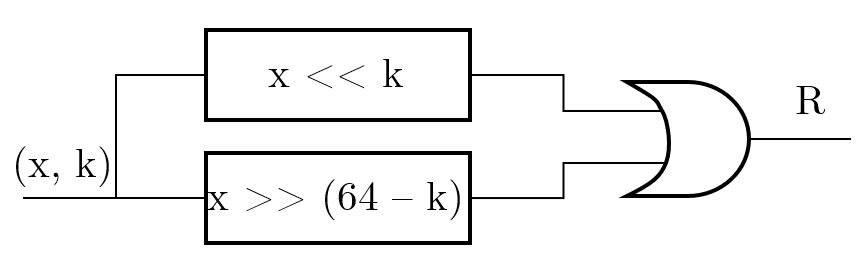
\includegraphics[width=0.6\textwidth]{xoroshiro_rot.JPG}
    \centering
    \caption{Rotation in Xoroshiro}
    \label{fig:xoroshiro_rot}
\end{figure}

The algorithm is named after its routine of transformations being used. The core of the algorithm performs  \textit{XOR}, \textit{RO}tate, \textit{SHI}ft and \textit{RO}tate, which is the reason for the name. This routine is performed over two \acrfull{iv}s which will be replaced after transformation, to the next iteration. Random bit string would be the arithmetic sum of the IVs, before transformation.

Generator initialised with IVs $s_1$ and $s_2$. Each iteration begins by adding the current values of the IVs to generate the next bit string ($\varepsilon_i$). Then, $s_1$ is replaced by $s_1 \oplus s_2$, followed XOR with Rotation and Shifting is performed over $s_1$ and Rotation is performed over $s_2$. At the end of the iteration, the value $\varepsilon_i$ is returned.

\subsubsection{Statistical Quality and Performance}

According to the statements made by the authors, "\textit{It passes all tests we are aware of except for the four lower bits, which might fail linearity tests (and just those), so if low linear complexity is not considered an issue (as it is usually the case) it can be used to generate 64-bit outputs, too; moreover, this generator has a very mild Hamming-weight dependency making our test (http://prng.di.unimi.it/hwd.php) fail after 8 TB of output; we believe this slight bias cannot affect any application} \cite{web_xoroshiro_impl}.

The algorithm has a $2^{128}$ period which is comparatively much less than that of the MT. Yet, it is capable of generating pseudorandom numbers at a rate which is as high as 1.2 nanoseconds per 64-bit number as claimed by Matt Gallagher, in his study on random number generators in Swift \cite{web_xoroshiro_mg_swift}. The statistical results have been verified in both PractRand and TestU01 by the authors. 

\section{Environmental Randomness}

As Linus Trovalds outlines in the documenting comments of the source code of \ilcode{/dev/random} and \ilcode{/dev/urandom} "\textit{Computers are very predictable devices.  Hence it is extremely hard to produce truly random numbers on a computer --- as opposed to pseudo-random numbers, which can easily generated by using an algorithm. Unfortunately, it is very easy for attackers to guess the sequence of pseudo-random number generators, and for some applications this is not acceptable.  So instead, we must try to gather "environmental noise" from the computer's environment, which must be hard for outside attackers to observe, and use that to generate random numbers.  In a Unix environment, this is best done from inside the kernel.}\cite{web_random_c_git}

Here, the term \textit{Environmental Noise} is an interesting topic. By the same, it is referred to the internal environment of a computer, which is composed of the hardware platform and the OS platform. However for the case of this study, this concept of environment has further extended up to the surrounding environment. According to Trovalds, the sources used in the above random generators were chosen carefully to demonstrate the following attributes.

\begin{itemize}
    \item Non-deterministic
    \item Difficult for an outside observer to access
\end{itemize}

The first attribute above traces back to the characteristics of true randomness outlined previously in subsection \ref{subsec:rand_attr_sum}. Furthermore, the idea of difficulty for an outsider to observe, is a relative matter which depends on how much information and probes are available to the said observer. In that sense, to the eye of an outside observer who does not possess sufficient information and probes to access a particular system, the system might appear truly random, given that the system demonstrates other characteristics of true randomness. This leads to the fact that true randomness in the current context, is relative.

\section{Evaluation of Randomness}

When choosing a source, model or a system that generates random data, it is primarily important to determine its quality of randomness. This would require different metrics of quality. To compare between many different sources of randomness for their quality, it is important that these metrics be comparable. This essentially emphasises the fact that these metrics should be quantitative and objective.

It is possible to find a handful of practical measures and tests of randomness of a binary string. Almost all of these tests include measures which are based on statistical tests, different sorts of transforms and complexity or a combination of these types. For instances one could consider the use of Hadamard transform that measures randomness. This suite was proposed by S. Kak and further developed by Phillips, Yuen, Hopkins, Beth and Dai, Mund, and Marsaglia and Zaman\cite{web_rand_tests_lit}.

Among the available tests, the publication with the title "\textit{A Statistical Test Suite for Random and Pseudorandom Number Generators for Cryptographic Applications}" published by the \acrshort{nist} under the publication number \acrshort{nist} Special Publication 800-22, appears to have gained wider acceptance throughout the community. This document provides a detailed elaboration of a collection of statistical tests which could be performed over a given potential input data. These tests, according to \acrshort{nist} could be used in different combinations to evaluate the quality of randomness of the input.

\subsection{BSI Evaluation Criteria}

The Federal Office for Information Security (Bundesamt für Sicherheit in der Informationstechnik, BSI) Germany, has established a four-fold criteria to asses and rank the quality of deterministic random number generators\cite{art_schindler_eval_meth}. Those could be summarized as follows.

\begin{itemize}
    \item \textbf{K1} – The probability of generated sequences of random numbers being different from each other should be high.
    \item \textbf{K2} – A sequence of numbers which is indistinguishable from 'true random' numbers according to specified statistical tests. These tests should include
    
        \begin{enumerate}
            \item Monobit test (equal numbers of ones and zeros in the sequence)
            \item Poker test (a special instance of the chi-squared test)
            \item Runs test (counts the frequency of runs of various lengths)
            \item Longruns test (checks whether there exists any run of length 34 or greater in 20 000 bits of the sequence)—both from BSI and NIST
            \item Auto correlation test
        \end{enumerate}
    
    In essence, these requirements are a test of how well a bit sequence: has zeros and ones equally often; after a sequence of n zeros (or ones), the next bit a one (or zero) with probability one-half; and any selected subsequence contains no information about the next element(s) in the sequence.
    \item \textbf{K3} – It should be impossible for any attacker (for all practical purposes) to calculate, or otherwise guess, from any given subsequence, any previous or future values in the sequence, nor any inner state of the generator.
    \item \textbf{K4} – It should be impossible, for all practical purposes, for an attacker to calculate, or guess from an inner state of the generator, any previous numbers in the sequence or any previous inner generator states.
\end{itemize}

For cryptographic applications, generators which are meeting the K3 or K4 standard only would be accepted.

\subsection{Unpredictability}

NIST emphasizes that \textit{Random and pseudorandom numbers generated for cryptographic applications should be unpredictable}\cite{rep_nist_sp_80022}. Further, it spans the discussion towards PRNGs and highlights the fact that given that the seed of a PRNG is kept a secret, next output number of the sequence should be unpredictable, in spite of any knowledge of the previous random numbers. This is identified as \textit{forward unpredictability}. Along with that, it is also important that, given the entire or a part of the sequence of random numbers generated is known, it should be infeasible to determine the seed used for the given sequence. This attribute is known as \textit{backward unpredictability}. There should not be any obvious or computable correlation between the seed and any of the random numbers in the sequence \cite{rep_nist_sp_80022}.

\subsection{Statistical Tests Suite of NIST}

NIST, in their special publication 800-22 highlights that there is a variety of statistical tests that could be applied to a random sequence to compare and evaluate the sequence for its randomness. Randomness is a probabilistic property; i.e., the attributes of any random sequence can be characterised and described in terms of probability. The probable outcome of any statistical evaluation, when applied on a truly random sequence, is known \textit{a priori} and can be described in probabilistic terms. There are infinitely many statistical tests that could be utilised that which each is evaluating the presence or absence of a pattern which, if identified, would indicate that the sequence is not random. Since there is an abundance of tests for evaluating the randomness and its degree of a given sequence, it is not possible to deem that \textit{this finite set of tests is deemed "complete"} \cite{rep_nist_sp_80022}.

Apart from that, SP 800-22 also highlights that the results of statistical testing on a random sequence must be interpreted with due care and caution to avoid possible incorrect conclusions about a specific generator \cite{rep_nist_sp_80022}. According to NIST, how the test results should be interpreted is extremely sensitive to the sequence and its utilisation. This matter is discussed in detail later under this section.

A statistical test is specifically composed to evaluate a predetermined \textit{Null Hypothesis} ($H0$). In the test suite given by NIST, the null hypothesis being tested is that \textit{the sequence being tested is random}. There is an \textit{Alternative Hypothesis} ($Ha$) associated with this null hypothesis, which in the test suite, is that \textit{the sequence is not random}. For each of the test which is conducted, a decision or conclusion is derived for \textit{whether to accept or reject the null hypothesis}, i.e., whether the generator is or is not producing a random sequence.

For each of tests taken, an applicable randomness statistic should be chosen and used to derive whether the null hypothesis is accepted or rejected. Under an assumption of randomness, such a statistic would have a distribution of possible values. A theoretical reference distribution for the chosen statistic under the null hypothesis would be determined by different mathematical methods. From reference distribution derived, a \textit{critical value} is determined. In most of the cases, the critical value is "far out" towards the tail of the reference distribution, say out at the $99^{th}$ percentile. During a test, a test statistic value is computed on the sequence that is being tested. Then the calculated test statistic value is compared against the critical value for the particular test. If the test statistic value obtained exceeds the critical value, the null hypothesis for randomness will be rejected. Otherwise, the null hypothesis accepted.

In practice, the reason why the statistical hypothesis testing works is that the reference distribution and the critical value are dependent on and generated under a tentative assumption of randomness. If the randomness assumption is, in fact, true for the data at hand, then the resulting test statistic value on the data will have a very low probability (e.g., 0.01\%) of exceeding the critical value. On the other hand, if the calculated test statistic value does exceed the critical value (i.e., if the low probability event does in fact occur), then from a statistical hypothesis testing perspective, the low probability event should not occur naturally. Hence, when the calculated test statistic value exceeds the critical value for the given test, it is arrived at the conclusion that the original assumption of randomness is suspicious or faulty. In this case, statistical hypothesis testing yields the conclusions of  rejecting $H0$ (randomness) and accepting $Ha$ (non-randomness) \cite{rep_nist_sp_80022}.

Statistical hypothesis testing is a procedure of generating conclusions that which possible outcomes are two folded. Those are namely

\begin{enumerate}
    \item Accept $H0$ (the data is random)
    \item Accept $Ha$ (the data is non-random)
\end{enumerate}

The relating of the true (unknown) status of the data at hand to the conclusion arrived at using the testing procedure could be tabulated as follows (Table \ref{tbl_hypothesis}).

\begin{table}[h!]
\centering
    \begin{tabular}{ |c|c|c| } 
        \hline
        \multirow{2}{*}{TRUE SITUATION} & \multicolumn{2}{|c|}{CONCLUSION} \\
        \cline{2-3}
        & Accept $H0$ & Accept $Ha$ (reject $H0$) \\
        \hline
        Data is random ($H0$ is true) & No error & Type I error \\
        \hline
        Data is not random ($Ha$ is true) & Type II error & No error \\
        \hline
    \end{tabular}
    \caption{Conclusions on Each Hypothesis\cite{rep_nist_sp_80022}}
    \label{tbl_hypothesis}
\end{table}

If the data in the sequence is random, then a conclusion to reject the null hypothesis (i.e., to conclude that the data stream is not random) might occur during a small percentage of the time. If it is arrived at such conclusion, it is called a \textit{Type I error}. If the data in the sequence is actually not random, then if it reaches at a conclusion to accept the null hypothesis (i.e., to accept that the data is actually random) is called a \textit{Type II error}. The conclusions to accept $H0$ when the data is really random, and to reject $H0$ when the data is non-random, are correct.

The probability of Type I error is occurring is often called the \textit{level of significance} of the test. This probability could be set prior to a test and is denoted as $\alpha$. For any of the tests, $\alpha$ denotes the probability that the test will indicate that the sequence is not random when it really is random i.e., a sequence appears to have non-random properties even when a “good” generator produced the sequence. Most commonly, values of $\alpha$ in cryptography lies about $0.01$.

The probability of a Type II error is denoted by $\beta$. For any of the tests, $\beta$ is the probability that the test would indicate that the sequence is random when it is actually not i.e., a "bad" generator that produces a sequence which appears to demonstrate attributes of quality randomness. Unlike $\alpha$, $\beta$ would not be a fixed value. $\beta$ could take on many different values because there are an infinitely many number of permutations that a data stream can be not random, and each different way yields a different $\beta$. Computation of the Type II error $\beta$ is quite difficult than the calculation of $\alpha$ because of the many different possibilities of types of non-randomness.

One of the primary goals of the tests enumerated below is to minimise the probability of a Type II error, i.e., to minimise the probability of accepting a sequence being produced by a generator as good when the generator is actually of low quality. The probabilities $\alpha$ and $\beta$ are related mutually and also to the size $n$ of the sequence being tested in such a way that when two of those values are specified, the third value could automatically be determined. Practitioners generally choose a sample size $n$ and a value for $\alpha$ i.e. the probability of a Type I error/the level of significance. Then a critical value for a given statistic is chosen in such a way that will produce the smallest $\beta$ i.e. the probability of a Type II error. That is, a suitable sample size is selected along with an acceptable probability of deciding if a bad generator has produced the sequence when it really is random. Then the cutoff point for acceptability would be chosen in such a way that the probability of falsely accepting a sequence as random has the smallest possible value.

Each of the tests is based on a calculated test statistic value, which is a function of the data. If the test statistic value is S and the critical value is t, then the Type I error probability is 

\[
    P(S > t \parallel H0 \text{ is true}) = P(\text{reject } H0 \mid H0 \text{ is true})
\]

and the Type II error probability is

\[
    P(S \leq t \parallel H0 \text{ is false}) = P(\text{accept } H0 \mid H0 \text{ is false})
\]

The test statistic is used to calculate a $P$-value that summarises the strength of the evidence which are against $H0$. For these tests, each $P$-value is the probability that a perfect random number generator would have produced a sequence, which is less random than the sequence that was tested, given the kind of non-randomness assessed by the test. If a $P$-value for a test is determined to be equal to 1, then the sequence being tested appears to have perfect randomness. A $P$-value of zero indicates that the sequence appears to be completely non-random. A significance level ($\alpha$) can be chosen for the tests. If $P$-value is less than or equal to $\alpha$, then $H0$ is accepted i.e., the sequence appears to be random. If $P$-value is greater than $\alpha$, then $H0$ is rejected i.e., the sequence appears to be non-random. The parameter $\alpha$ denotes the probability of the Type I error. Typically, $\alpha$ is chosen in the range [0.001, 0.01] \cite{rep_nist_sp_80022}.

\begin{itemize}
    \item An $\alpha$ of 0.001 indicates that one would expect one sequence in 1000 sequences to be rejected by the test even if the sequence was random. For $P \geq 0.001$, a sequence would be considered to be random with a confidence of 99.9\%. For $P < 0.001$, a sequence would be considered to be nonrandom with a confidence of 99.9\% \cite{rep_nist_sp_80022}.
    
    \item An $\alpha$ of 0.01 indicates that one would expect 1 sequence in 100 sequences to be rejected. $P \geq 0.01$ would mean that the sequence would be considered to be random with a confidence of 99\%. $P < 0.001$ would mean that the conclusion was that the sequence is non-random with a confidence of 99\% \cite{rep_nist_sp_80022}.
\end{itemize}

\section{Testing Strategy of NIST Statistical Test Suite}

The following subsections are dedicated to closely review the mathematical foundation of the tests which are included in this test suite.

\subsection{Frequency (Monobits) Test}\label{subsec:monobits}

This is the most basic test which has the null hypothesis of \textit{in a sequence of independent identically distributed Bernoulli random variables ($X$'s or $\varepsilon$'s, where $X =2_{\varepsilon}-1$, and so $S_n = X_1 + \ldots + X_n = 2(\varepsilon_1 + \ldots + \varepsilon_n) – n)$, the probability of ones is 1/2}. By the classic \textit{De Moivre-Laplace theorem}, for an adequately large number of trials, the distribution of the normalised binomial sum by $\sqrt{n}$ , can be reasonably attributed to a standard normal distribution. This test makes use of that approximation to assess the closeness of the fraction of 1's to 1/2. All subsequent tests are conditioned on having passed this first basic test.

This test is derived from the well-known \textit{Central Limit Theorem} for the random walk, $S_n = X+1 + \ldots + X_n$. As per the Central Limit Theorem,
\[
    \lim_{n\to\infty} P(\dfrac{S_n}{\sqrt{n}} \leq z) = \Phi(z) \equiv \dfrac{1}{\sqrt{2\pi}}\int_{-\infty}^{z}e^{-u^2/2} du
\]

This classical result serves as the basis of the simplest test for randomness. It implies that, for $z \in \mathbb{Z}^+$,
\[
    P(\dfrac{\lvert S_n \rvert}{\sqrt{n}} \leq z) = 2\Phi(z) - 1
\]

According to the test based on the statistic $s = \lvert S_n \rvert / \sqrt{n}$, evaluate the observed value $\lvert s(obs) \rvert = \lvert X_1 + \ldots + X_n \rvert / \sqrt{n}$, and then calculate the corresponding P-value, which is $2[1 - \Phi(\lvert s(obs) \rvert)] = efrc(\lvert s(obs) \rvert)/\sqrt{n}$. Here, $erfc$ is the (complementary) error function

\[
\textit{erfc}(z) = \dfrac{2}{\sqrt{\pi}}\int_{z}^{\infty}e^{-u^2} du
\]

\subsubsection{Implementation}

This test could be implemented using a function $frequency(n)$ where $n$ is the length of the bit string being tested. Additionally, the code should have access to $\varepsilon$, which is the bit string generated by the RNG being tested (i.e. $\varepsilon = \varepsilon_1, \varepsilon_2, \ldots, \varepsilon_n; \forall \varepsilon \in \mathbb{F}_2$). Test statistic would be $S_{\text{abs}}$ which is the absolute value of the sum of $X_i$ where $X_i = 2\varepsilon_i - 1$, divided by $\sqrt{n}$.

If $z = S_{\text{abs}} / \sqrt{2}$ is distributed normal, then $\lvert Z \rvert$ should be \textit{half normal}. Hence, the reference distribution for the test statistic should be \textit{half normal} for large $n$. If the number of 0's and 1's are absolutely the same, then the test statistic would be zero. Therefore, closer the test statistic to zero, better it would be.

The test should be implemented as per the steps enumerated below.

\begin{enumerate}
    \item Convert bits of the string to $\pm 1$ with $2\varepsilon_i - 1$. (E.g. if $\varepsilon = 1011010101$, then $n=10$ and $S_n = 1 + (-1) + 1 + 1 + (-1) + 1 + (-1) + 1 + (-1) + 1 = 2$)
    
    \item Compute the test statistic $S_{\text{abs}} = \dfrac{\lvert S_n \rvert}{\sqrt{n}}$. (E.g. $S_{\text{abs}} = \dfrac{\lvert 2 \rvert}{\sqrt{10}} = 0.632455532$)
    
    \item Compute $P$-value = $\text{efrc}(z)$ where $z = \dfrac{S_{\text{abs}}}{\sqrt{2}}$ and $\text{efrc}$ is the \textit{Complementary Error Function}. (E.g. $P = \text{efrc}(0.632455532 / \sqrt{2} = 0.527089)$).
\end{enumerate}

If the computed $P$-value is $< 0.01$, then it is concluded that the sequence being tested is not random. Very small $P$-values (i.e. $< 0.01$) are caused by large $\lvert S_n \rvert$ or $\lvert S_\text{abs} \rvert$. These two would be large, when the difference between the number of 1's and 0's gets larger in size.

As per the report from NIST, it is recommended that the input size should be \textit{at least 100 bits long} (i.e. $n \geq 100$).

\subsection{Frequency Test within a Block}

This test attempts to detect if there are any \textit{localised deviations} from the ideal 50\% frequency of 1's. This is attained by slicing the test sequence into non-overlapping sub-sequences and applying a \textit{chi-square test} for a homogeneous match of empirical frequencies to the ideal 50\%. Small P-values indicate large deviations from the equal proportion of ones and zeros in at least one of the substrings. The string of 0's and 1's (or equivalent -1's and 1's) is sliced into disjoint substrings. Then for each substring, the proportion of ones is computed. Then a chi-square statistic compares these substring proportions to the ideal 50\%.

The statistic is referred to a chi-squared distribution with the degrees of freedom equal to the number of substrings. The parameters of this test would be $M$ and $N$ such that $n = MN$, i.e., the original string is partitioned into $N$ number of substrings, each having $M$ number of bits. For each of these substrings, the probability of ones is estimated by the observed relative frequency of 1's, $\Phi_i$, ${i | i \in \mathbb{Z}^+; i \leq N}$. The sum

\[
    \chi^2(\text{obs}) = 4M\sum_{i=1}^{N}\bigg[ \pi_i - \dfrac{1}{2}\bigg]^2
\]

under the randomness hypothesis has the $Χ^2$-distribution with N degrees of freedom. The reported $P$-value is
\[
    \dfrac{\int_{x^2_{\text{(obs)}}}^\infty e^{-u/2}u^{(N/2)-1} du}{\Tau(N/2)2^{N/2}} = \dfrac{9\int_{x^2_{\text{(obs)}/2}}^\infty e^{-u}u^{(N/2)-1} du}{\Tau(N/2)} = \text{igamc}(\dfrac{N}{2}, \dfrac{X^2(\text{obs})}{2})
\]

\subsubsection{Implementation}

Implementation of the test would be to deploy a function $blockFrequency(M,n)$, where $M$ is the length of each block and $n$ is the length of the bit string being tested. Additionally, the code should have access to $\varepsilon$, which is the bit string generated by the RNG being tested (same as Subsection \ref{subsec:monobits}). Test statistic would be $\chi^2_\text{(obs)}$, which is a measure of how well the observed proportions of ones within a given M-bit block match the expected proportion (1/2). The reference distribution for the test statistic would be a $\chi^2$ distribution\cite{rep_nist_sp_80022}.

Following process is to be followed to implement the test.

\begin{enumerate}
    \item Partition the input sequence into $N = \floor*{\dfrac{n}{M}}$ \textit{non-overlapping} blocks. Low-order bits which are not grouped are to be discarded. (E.g. if $n = 10$, $M = 3$ and $\varepsilon = 0110011010$, 3 blocks ($N = 3$) would be created, consisting of $011$, $001$ and $101$. $0$ at the end will be discarded.)
    
    \item Determine $\pi_i$ (proportion of 1's in each M-bit block) using $\pi_i = \dfrac{\sum_{j=1}^{M}\varepsilon_{(i-1)M+j}}{M}$, for $1 \le i \le N$. (E.g. $\pi_1 = 2/3$, $\pi_2 = 1/3$, and $\pi_3 = 2/3$.)
    
    \item Compute $\chi^2_{\text{obs}} = 4M\sum_{i=1}^{N}\bigg[ \pi_i - \dfrac{1}{2}\bigg]^2$. (E.g. $\chi^2_{\text{obs}} = 1$)
    
    \item Compute $P\text{-value}  = \text{igamc}(\dfrac{N}{2}, \dfrac{X^2(\text{obs})}{2})$, where $\text{igamc}$ is the \textit{Incomplete Gamma Function} for $Q(a,x)$. (Note: $Q(a,x) = 1 = P(a,x)$) (E.g. $P\text{-value} = \text{igamc}(3/2, 1/2) = 0.801252$)
\end{enumerate}

Small $P$-values ($< 0.01$) indicates a large deviation from the equal proportion of 1's and 0's in at least one block. For the inputs, size of the input should at least be 100 bits (i.e. $n \ge 100$). $M$ and $N$ should be chosen such that $MN \le n$ where ideally, $M > 0.1n$ and $N < 100$.

\subsection{Runs Test}

This variant of a classic non parametric test looks at “runs” defined as substrings of consecutive 1's and consecutive 0's, and considers whether the oscillation among such homogeneous substrings is too fast or too slow. The specific test used here is based on the distribution of the total number of runs, $V_n$. For the fixed proportion $\pi = \dfrac{\sum_j \varepsilon_j}{n}$ (which by the Frequency (Mono bits) Test (Subsection \ref{subsec:monobits}) must have been established to be close to 0.5: $\lvert \pi - \dfrac{1}{2} \rvert \leq \dfrac{2}{\sqrt{n}}$) \cite{rep_nist_sp_80022}.

\[
        \lim_{x\to\infty} P \bigg(\dfrac{V_n - 2n\pi(1-\pi)}{2\sqrt{n}\pi(1-\pi)} \leq z\bigg) = \Phi(z)
\]

To evaluate $V_n$, define for $k \in \mathbb{Z}_i; 1 \leq i \leq n-1$, $r(k) = 0$ if $\varepsilon_k = \varepsilon_{k+1}$ and $r(k) = 1$ if $\varepsilon_k \ne \varepsilon_{k+1}$. Then $V_n = \sum_{k=1}^{n-1}r(k) + 1$. The $P$-value is reported as

\[
    \text{erfc}(\dfrac{\lvert V_n(\text{obs}) - 2n\pi(1-\pi)\rvert}{2\sqrt{2n}\pi(1-\pi)})
\]

As per the NIST report, large values for $V_n(\text{obs})$ would indicate that the oscillation in the string of $\varepsilon$'s which is too fast. Samll values for such would indicate that the oscillation is too slow.

\subsubsection{Implementation}

Implementation is to deploy a function $runs(n)$, where $n$ is the length of the bit string. Also, the code should have access to $\varepsilon$, which is the bit string generated by the RNG being tested (same as in Subsection \ref{subsec:monobits}). $V_n(\text{obs})$, which is the total number of runs (i.e. the total of 0 runs + the total of 1 runs) across all $n$ bits would be the test statistic which refers to a $\chi_2$ distribution. Implementation steps would be as follows.

\begin{enumerate}
    \item Compute $\pi$, the pretest proportion of 1's in the sequence with $\pi = \dfrac{\sum_j \varepsilon_j}{n}$ (E.g. if $\varepsilon = 1001101011$, then $n = 10$ and $\pi = 6/10 = 3/5$).
    
    \item Determine if the prerequisite Frequency test is passed. If it could be determined that $\lvert \pi - 1/2 \rvert \geq \tau$ (where $\tau = \dfrac{2}{\sqrt{n}}$), then this test need not to be performed (i.e. the test should not have been run because of a failure to pass the test 1, the Frequency Test). If the test is not applicable, then the $P$-value is set to 0.0. (E.g. since $\tau = 2\sqrt{10} \approx 0.63246$, then $\lvert \pi - 1/2 \rvert = \lvert 3/5 - 1/2 \rvert = 0.1 < \tau$, and the test is not run. Since the observed value of $\pi$ is within the selected bounds, the runs test is applicable.)
    
    \item Compute the statistic $V_n(\text{obs}) = \sum_{k=1}^{n-1}r(k) + 1$, where $r(k) = 0$ if $\varepsilon_k = \varepsilon_{k+1}$ and $r(k) = 1$ if $\varepsilon_k \ne \varepsilon_{k+1}$.  (E.g. Since $\varepsilon = 1001101011$, $V_{10}(\text{obs}) = (1+0+1+0+1+1+1+1+0)+1=7$).
    
    \item Compute the $P$-value with $\text{erfc}(\dfrac{\lvert V_n(\text{obs}) - 2n\pi(1-\pi)\rvert}{2\sqrt{2n}\pi(1-\pi)})$. (E.g. in the above, $P\text{-value} = 0.147232$).
\end{enumerate}

If the computed $P$-value is $< 0.01$, then it is concluded that the sequence is non-random. Otherwise, it is concluded that the sequence is random. Note that a large value for $V_n(\text{obs})$ would have indicated an oscillation in the string which is too fast and a small value would have indicated that the oscillation is too slow. (An oscillation is considered to be a change from a one to a zero or vice versa.) A fast oscillation occurs when there are a lot of changes, e.g., 010101010 oscillates with every bit. A stream with a slow oscillation has fewer runs than would be expected in a random sequence, e.g., a sequence containing 100 ones, followed by 73 zeroes, followed by 127 ones (a total of 300 bits) would have only three runs, whereas 150 runs would be expected\cite{rep_nist_sp_80022}. The recommended input size for this test is a minimum of 100 bits (i.e. $n \geq 100$).

\subsection{Test for the Longest Run of Ones in a Block}

The length of the longest consecutive sub sequence (run) of ones is another characteristic that can be used to determine the degree of randomness. A string of length $n$, such that $n = MN$, is to be partitioned into $N$ substrings, each of length $M$. For the test based on the length of the longest run of ones $\nu_j$ within the $j^{\text{th}}$ substring of size $M$, $K + 1$ classes are chosen based on $M$. For each of these substrings, one evaluates the frequencies $\nu_i;0\leq i \leq k$($\sum_{i=0}^{k}\nu+i = N$ , i.e., the computed values of the longest run of ones within each of these substrings belonging to any of the $K + 1$ chosen classes). If there are $r$ ones and $M-r$ zeroes in the $m$-bit block, then the conditional probability that the longest string of ones $\nu$ in this block is less than or equal to $m$, would take the following form with $U = \text(min)(M - r + 1, \bigg[\dfrac{r}{m + 1}\bigg])$.

\[
    P(v \leq m) = \sum_{r=0}^{M} \begin{pmatrix}M \\ r\end{pmatrix}P(v \leq m | r) \dfrac{1}{2^M}
\]

The theoretical probabilities $\pi_0, \pi_1, \ldots, \pi_k$ of these classes are determined from the above summation. The empirical frequencies $\nu_i; 0 \geq i \geq k$are conjoined by $X^2$ statistic

\[
    X^2 = \sum_{i=0}^{K} \dfrac{(V_i - N\pi_i)^2}{N\pi_i}
\]
which, under the randomness hypothesis, has an approximate $Χ^2$ -distribution with $K$ degrees of freedom. The reported P-value is

\[
    \dfrac{\int_{X^2_{\text{(obs)}}}^\infty e^{-u/2}u^{(K/2)-1} du}{\Tau(K/2)2^{K/2}} = \text{igamc}\bigg(\dfrac{K}{2}, \dfrac{X^2(\text{obs})}{2}\bigg)
\]
with $P(a,x)$ denoting the incomplete gamma function as expressed previously. Table below (table \ref{tab:class_prob_38}) specifies the count classes and the probabilities for the case where $K = 3$ and $M = 128$. Other for other combinations also, there are predetermined classes and corresponding probability values available in the test suite.

    \begin{table}[h!]
        \centering
        \begin{tabular}{|c|c|} \hline
            \textbf{classes} & \textbf{probabilities} \\ \hline
            \textbf{$\nu \leq 4$} & $\pi_0 = 0.1174$ \\ \hline
            \textbf{$\nu = 5$} & $\pi_1 = 0.2430$ \\ \hline
            \textbf{$\nu = 6$} & $\pi_2 = 0.2493$ \\ \hline
            \textbf{$\nu = 7$} & $\pi_3 = 0.1752$ \\ \hline
            \textbf{$\nu = 8$} & $\pi_4 = 0.1027$ \\ \hline
            \textbf{$\nu  \geq 9$} & $\pi_5 = 0.1124$ \\ \hline
        \end{tabular}
        \caption{Count classes and Probabilities ($K=3, M=8$)}
        \label{tab:class_prob_38}
    \end{table}

\subsubsection{Implementation}

Execution of the test requires implementing a function $longestRunOfOnes(n)$ that which takes $n$ which is the length of the input string as a parameter along with access to $\varepsilon$ which is the generated string by the RNG as an internal parameter. Also it would need to have $M$ which is the length of a block. This should be taken in relation to $n$ as mentioned below (table \ref{tab:sb_length_for_n}).

    \begin{table}[h!]
        \centering
        \begin{tabular}{|c|c|} \hline
             \textbf{Minimum $n$} & \textbf{M}  \\ \hline
             \textbf{128} & 8 \\ \hline
             \textbf{6272} & 128 \\ \hline
             \textbf{750000} & $10^4$ \\ \hline
        \end{tabular}
        \caption{Recommended sub-block length for each string size}
        \label{tab:sb_length_for_n}
    \end{table}
    
Test statistic would be $\chi^2_\text{(obs)}$, which is a measure of how well the observed longest run length with $M$-bit blocks matches the expected longest length within $M$-bit blocks, which refers to a $\chi^2$ distribution. Test routine should be as follows.

\begin{enumerate}
    \item Divide the sequence into $M$-bit blocks,
    \item Tabulate the frequencies $v_i$ of the longest runs of 1's of each block. This tabulation should be done as per the table given below (see Table \ref{tab:sb_freq_crit}).
    
    \begin{table}[h!]
        \centering
        \begin{tabular}{|c|c|c|c|} \hline
            \textbf{$v_i$} & \textbf{M = 8} & \textbf{M = 128} & \textbf{M = 104} \\ \hline
            \textbf{$v_0$} & $\leq 1$ & $\leq 4$ & $\leq 10$ \\ \hline
            \textbf{$v_1$} & 2 & 5 & 11 \\ \hline
            \textbf{$v_2$} & 3 & 6 & 12 \\ \hline
            \textbf{$v_3$} & $\geq 4$ & 7 & 13 \\ \hline
            \textbf{$v_4$} &  & 8 & 14 \\ \hline
            \textbf{$v_5$} &  & $\geq 9$ & 15 \\ \hline
            \textbf{$v_6$} &  &  & $\geq 16$ \\ \hline
        \end{tabular}
        \caption{Frequency counting criteria for sub-blocks}
        \label{tab:sb_freq_crit}
    \end{table}
    
    \item Compute $\chi^2_{\text{(obs)}} = \sum_{i=0}^{K} \dfrac{(V_i - N\pi_i)^2}{N\pi_i}$, with the predefined values for $\pi_i$ ($\pi_i$ to be obtained as stipulated in table \ref{tab:class_prob_38}). Values for $K$ and $N$ are stipulated as follows (table \ref{tab:kn_values}).
    
    \begin{table}[h!]
    \centering
        \begin{tabular}{|c|c|c|} \hline
        \textbf{M} & \textbf{K} & \textbf{N} \\ \hline
        8 & 3 & 16 \\ \hline
        128 & 5 & 49 \\ \hline
        $10^4$ & 6 & 75 \\ \hline
        \end{tabular}
        \caption{Value combinations for $K$ and $N$}
        \label{tab:kn_values}
    \end{table}
    
    \item Compute $P$-value with $\text{igamc}\bigg(\dfrac{K}{2}, \dfrac{\chi^2(\text{obs})}{2}\bigg)$
\end{enumerate}

Large values for $\chi^2_{\text{(obs)}}$ indicate that the tested sequence is having clusters of ones which are too large. Hence the $P$-value would be reduced. If the $P$-value is $\geq 0.01$, the sequence is accepted to be sufficiently random. Minimum length of the input string ($n$) is recommended to be as stipulated in table \ref{tab:sb_length_for_n}.

\subsection{Binary Matrix Rank Test}

This test focuses at the rank of \textit{disjoint sub matrices} of the entire sequence. The purpose of this test is to check for linear dependence among fixed length substrings of the original sequence. Note that this test also appears in the \textit{DIEHARD} battery of tests. To apply the $X^2$-test it uses the classical statistic

\[
    X^2 = \dfrac{(F_M  - 0.2888N)^2}{0.2888N} + \dfrac{(F_{M-1}  - 0.5776N)^2}{0.5776N} + \dfrac{(N - F_M - F_{M-1}  - 0.1336N)^2}{0.1336N}
\]
which under $H_0$ has an approximate $X^2$-distribution with 2 degrees of freedom. The reported $P$-value is $\text{exp}\bigg\{\dfrac{-X^2(\text{obs})}{2}\bigg\}$. Large values of $X^2(\text{obs})$ indicate that the deviation of the rank distribution from that corresponding to a random sequence is significant. For example, pseudo random matrices produced by a shift-register generator formed by less than $M$ successive vectors systematically have rank $R_l \equiv M$, while for truly random data, the proportion of such occurrences should be only about 0.29 \cite{rep_nist_sp_80022}.

\subsubsection{Implementation}

Execution of the test requires implementing a function $longestRunOfOnes(n)$ that which takes $n$ which is the length of the input string as a parameter along with access to $\varepsilon$ which is the generated string by the RNG as an internal parameter. Also it requires to set two other internal parameters $M$ and $N$ which are the number of columns and rows for the matrix, respectively. Both of these are set to 32 and the approximations which are specified in the NIST's test criteria is used. Test statistic would be $\chi^2_\text{(obs)}$, which is a measure of how well the observed number of ranks of various orders match the expected number of ranks under an assumption of randomness, which refers to a $\chi^2$ distribution. Test routine should be as follows.

\begin{enumerate}
    \item Sequentially divide the sequence to be tested, into $M \cdot Q$-bit blocks which are disjoint. There would be $N = \floor*{\dfrac{n}{MQ}}$ blocks. Remaining bits which would not fit into a block would be discarded.
    
    \item Collect and transform each block into a $M \times Q$ matrix.
    
    \item Determine the binary rank ($R_l; 1 \leq l \leq N$) for each matrix.
    
    \item Assign $F_M = $ the number of matrices with $R_l = M$ (full rank), $F_{M - 1}= $ the number of matrices with $R_l = M - 1$ (full rank - 1) and $N - F_{M} - F_{M - 1}= $ the number of matrices remaining.
    
    \item Compute 
    
    \[\scriptstyle
    X^2 = \dfrac{(F_M  - 0.2888N)^2}{0.2888N} + \dfrac{(F_{M-1}  - 0.5776N)^2}{0.5776N} + \dfrac{(N - F_M - F_{M-1}  - 0.1336N)^2}{0.1336N}
    \]
    
    \item Compute $P$-value $ = e^{-\chi^2\text{(obs)} / 2}$.
\end{enumerate}

Large values of $\chi^2\text{( obs )}$ (and hence, small $P$-values) would have indicated a deviation of the rank distribution from that corresponding to a random sequence is comparatively large. Hence the $P$-value would be $< 0.01$. As for the input size, the probabilities for $M = Q = 32$ have been predetermined and defined within the test routine. Other choices of $M$ and $Q$ may be selected, but the probabilities would need to be recalculated accordingly. The minimum number of bits to be tested must be such that $n \geq 38MQ$ so that there would be at least 38 matrices created from the input being tested. For $M = Q = 32$, each sequence to be tested should consist of \textit{a minimum of 38,912 bits}.

\subsection{Discrete Fourier Transform (Spectral) Test}

The test focuses on the peak heights in the \acrfull{dft} of the sequence. DFT is a member of a class of procedures known as \textit{spectral method}. The test would detect periodic features (i.e. certain repetitive patterns that are lying near each other) in the tested sequence that would indicate a deviation from the assumption of randomness. The intention is to detect whether the number of peaks exceeding the 95\% threshold is significantly different than 5\%.

Let $x_k; 1 \leq k \leq n$ be the $k^\text{th}$ bit of an input string of length $n$ and assume the bits $0$ and $1$ are coded $+1$ and $-1$ respectively. Then

\[
    f_j = \sum_{k=1}^{n} x_k exp(\dfrac{2\pi_i(k-1)j}{n})
\]
where $exp(\dfrac{2\pi_i(k-1)j}{n}) = \text{cos}(2\pi k j / n) + i\text{sin}(2\pi k j / n)$ for $0 \leq j \leq n-1$ and $i \equiv \sqrt{-1}$. Because of the symmetry of the real to complex value transformation, only the values from $0$ to $(n/2 - 1)$ are considered. If $\text{mod}_j$ is the modulus of the complex number $f_j$, a confidence level could be placed on the values of $\text{mod}_j$ under the assumption of the randomness of the series $x_i$. Precisely, 95\% of the values should be under $h$ where $h = \sqrt{\bigg(\text{log}\dfrac{1}{0.05}\bigg)n}$. A $P$-value based on this threshold could be derived from the binomial distribution. For the test, the $P$-value shall be obtained with $\text{erfc}\bigg(\dfrac{\lvert d \rvert}{\sqrt{2}}\bigg)$.

\subsubsection{Implementation}

Execution of the test requires implementing a function $\textit{discreteFourierTransform}(n)$ that which takes $n$ which is the length of the input string as a parameter along with access to $\varepsilon$ which is the generated string by the RNG as an internal parameter. Statistic for this test is denoted by $d$ which is the normalised difference between the observed and the expected number of frequency components that are beyond the 95\% threshold, that refers to the normal distribution. Test routine is as enumerated below.

\begin{enumerate}
    \item Convert bits of the string to $\pm 1$ with $2\varepsilon_i - 1$. (E.g. if $\varepsilon = 1011010101$, then $n=10$ and $S_n = 1 + (-1) + 1 + 1 + (-1) + 1 + (-1) + 1 + (-1) + 1 = 2$)
    
    \item Apply DFT, which will generate a sequence of complex variables that represents periodic components of the sequence of bits at different frequencies.
    
    \item Calculate $M = \text{modulus}(S´) \equiv |S'|$, where $S´$ is the substring consisting of the first $n/2$ elements in $S$, and the modulus function produces a sequence of peak heights.
    
    \item Compute $h = \sqrt{\bigg(\text{log}\dfrac{1}{0.05}\bigg)n}$, which is the 95\% peak height threshold, which under an assumption of randomness, $T$ should not exceed.
    
    \item Compute $N_0 = 0.95n/2$ which is the expected theoretical 95\% number of peaks.
    
    \item Compute $N_1$ which is the actual observed number of peaks in the $M$ that are less than $T$.
    
    \item Compute $d = \dfrac{(N_1 - N_0)}{\sqrt{n(.95)(.05)/4}}$
    
    \item Compute $P$-value with $\text{erfc}\bigg(\dfrac{\lvert d \rvert}{\sqrt{2}}\bigg)$.
\end{enumerate}

For the observation, $d$ value that is too low would indicate that there were too few peaks (less than 95\%) below $T$, and too many peaks (more than 5\%) above $T$. It is recommended to use an input string of a minimum of 1000 bits (i.e. $n \geq 1000$).

\subsection{Non Overlapping Template Matching Test}\label{subsec:notmt}

The test focuses on the number of occurrences of predetermined target strings. This test is intended to detect generators that produce significantly large number of occurrences of a given non periodic pattern. For this test and for the Overlapping Template Matching test in the next subsection, an $m$-bit window is used to search for a specific $m$-bit pattern. If the pattern is not found, the window slides one bit position forward (right in this case). If the pattern is found, the window is reset to the bit after the found pattern, and the search resumes. The test would reject any sequence, which are having very large or very small number of occurrences of common patterns. These periodic patterns are predefined in the test setup as \textit{templates}.

\subsubsection{Implementation}

Execution of the test requires implementing a function $\textit{nonOverlappingTemplateMatching}(m,n)$ that which takes $n$ which is the length of the input string as a parameter and $m$ which is the length of each template (i.e. the target string). Along with these, the code should have access to the following as internal parameters.

\begin{itemize}
    \item $\varepsilon$ - Generated string by the RNG
    \item $B$ - $m$-bit template to be matched, which is a string of 1's and 0's and no periodic
    \item $M$ - Length of the substring of $\varepsilon$ to be tested
    \item $N$ - Number of independent blocks (this is fixed at 8 for the test code)
\end{itemize}

Test statistic shall be $\chi^2(\text{obs})$ which is a measure of how well the observed number of template \textit{\textbf{hits}} matches the expected number of template \textit{\textbf{hits}} under the determined assumption of randomness. This statistic refers to a $\chi^2$  distribution. Test routine is as enumerated below.

\begin{enumerate}
    \item Partition the sequence into $N$ non overlapping blocks which are of size $M$.
    
    \item The search of matches begins by creating and $m$-bit window where $m$ is the length of the template. Then the bits of the sequence, which are within that window would be compared with the template. If the bit string within the window, matches the template $B$, the window will be slid to right by $m$ positions, after $W_j$ (number of times that template $B$ occurs within the block where $1 \leq j \leq N$) is incremented by one. If the bit string within the window doesn't match the template, the window will be slid to right by one. This is as elaborated in table \ref{tab:bit_wind_310} where $\varepsilon=10100100101110010110$, $m=3$ and $B=001$.
    
    \begin{table}[h!]
        \small
        \centering
            \begin{tabular}{|c|c|c|c|c|}
            \hline
            \multirow{2}{*}{\textbf{Bit Positions}} & \multicolumn{2}{c|}{\textbf{Block 1} (1010010010)} & \multicolumn{2}{c|}{\textbf{Block 2} (1110010110)} \\ \cline{2-5} 
             & \textbf{Bits} & \textbf{$W_1$} & \textbf{Bits} & \textbf{$W_2$} \\ \hline
            \textbf{1-3} & 101 & 0 & 111 & 0 \\ \hline
            \textbf{2-4} & 010 & 0 & 110 & 0 \\ \hline
            \textbf{3-5} & 100 & 0 & 100 & 0 \\ \hline
            \textbf{4-6} & 001(hit) & Increment to 1 & 001 & Increment to 1 \\ \hline
            \textbf{5-7} & Not examined &  & Not examined &  \\ \hline
            \textbf{6-8} & Not examined &  & Not examined &  \\ \hline
            \textbf{7-9} & 001 & Increment to 2 & 011 & 1 \\ \hline
            \textbf{8-10} & 010(hit) & 2 & 110 & 1 \\ \hline
        \end{tabular}
        \caption{Examination proceed for $\varepsilon=10100100101110010110$, $m=3$ and $B=001$}
        \label{tab:bit_wind_310}
    \end{table}
    
    \item Under an assumption of randomness, compute the theoretical mean $\mu = \dfrac{M-m+1}{2}$ and variance $\sigma^2 = M\bigg(\dfrac{1}{2^m}-\dfrac{2m-1}{2^{2m}}$
    
    \item Compute $\chi^2(\text{obs}) = \sum_{j=1}^{N}\dfrac{(W_j-\mu)^2}{\sigma^2}$.
    
    \item Compute $P$-value with $\text{igamc}\bigg(\dfrac{N}{2}, \dfrac{\chi^2(\text{obs})}{2}\bigg)$
\end{enumerate}

Minute values of $P$-value ($< 0.01$) indicate that the sequence has irregular occurrences of possible template patterns, which would yield the test case to be non random. Test code has templates built-in for $\{m \in \mathbb{Z}|2 \leq m \leq 10\}$. Nonetheless, it is recommended that $m=9$ or $m=10$ in order to obtain meaningful results. Test code has $N=8$, which could be altered under the condition that $N \leq 100$ to assure that the resultant $P$-values are valid. Also, it is noted that $M > 0.01n$ and $N = \floor*{\dfrac{n}{M}}$.

\subsection{Overlapping Template Matching Test}

This test is as same as the previously discussed test in subsection \ref{subsec:notmt} except that the shifting of the $m$-bit window will always be by 1 bit.

\subsubsection{Implementation}

Execution of the test requires implementing a function $overlapTemplMatch(m,n)$ that which takes $n$ which is the length of the input string as a parameter and $m$ which is the length of each template (i.e. the target string). Along with these, the code should have access to the following as internal parameters.

\begin{itemize}
    \item $\varepsilon$ - Generated string by the RNG
    \item $B$ - $m$-bit template to be matched, which is a string of 1's and 0's and no periodic
    \item $K$ -  The degree of freedom. (Note: The test suite has a fixed value for this set to 5)
    \item $M$ - Length of the substring of $\varepsilon$ to be tested
    \item $N$ - Number of independent blocks (this is fixed at 8 for the test code)
\end{itemize}

Test statistic shall be $\chi^2(\text{obs})$ which is a measure of how well the observed number of template \textit{\textbf{hits}} matches the expected number of template \textit{\textbf{hits}} under the determined assumption of randomness. This statistic refers to a $\chi^2$  distribution. Test routine is as enumerated below.

\begin{enumerate}
    \item Partition the sequence into $N$ non overlapping blocks which are of size $M$. (E.g.  $\varepsilon=10111011110010110100011100101110111110000101101001$, where $n = 50$. When $K = 2$, $M = 10$ and $N = 5$ the five blocks would be $1011101111$, $0010110100$, $0111001011$, $1011111000$, and $0101101001$)
    
    \item Count the number of occurrences of $B$ in each of the $N$ blocks. The search begins with defining a $m$-bit window for the sequence that which the substring of bits within the window will be compared against the template $B$. If it matches the template, a primary counter $C_B$ will be increased. After increasing the primary counter, the window will be slid to right over one bit position. This will be repeated until the end of the string. Once the substring is completed, the counter array $\{\nu_i|i \in \mathbb{Z} \land 0 \leq i \leq 5\}$ such that $\nu_0$ is incremented when there are no occurrences of $B$ in a substring, $\nu_1$ is incremented for one occurrence of $B$ and so forth and $\nu_5$ is incremented for 5 or more occurrences of $B$. Dry run of this algorithm is tabulated in table \ref{tab:bit_wind_21050} below.
    
    \begin{table}[]
        \centering
        \begin{tabular}{|c|c|c|}
        \hline
        \textbf{Bit Position} & \textbf{Bit String at the Position} & \textbf{$C_B$} \\ \hline
        \textbf{1-2} & 10 & 0 \\ \hline
        \textbf{2-3} & 01 & 0 \\ \hline
        \textbf{3-4} & 11 (hit) & 1 \\ \hline
        \textbf{4-5} & 11 (hit) & 2 \\ \hline
        \textbf{5-6} & 10 & 2 \\ \hline
        \textbf{6-7} & 01 & 2 \\ \hline
        \textbf{7-8} & 11 (hit) & 3 \\ \hline
        \textbf{8-9} & 11 (hit) & 4 \\ \hline
        \textbf{9-10} & 11 (hit) & 5 \\ \hline
        \end{tabular}
        \caption{Counting routine for 10-bit block $1011101111$ with $m=2$ and $B=11$}
        \label{tab:bit_wind_21050}
    \end{table}
    Thus, after examining block 1, since there are 5 occurrences of $11$, $\nu_5$ is incremented, and $\nu_0 = 0$, $\nu_1 = 0$, $\nu_2 = 0$, $\nu_3 = 0$, $\nu_4 = 0$, and $\nu_5 = 1$. Likewise, once all 5 blocks are examined, the counters for the above example would take the shapes of $\nu_0 = 0$, $\nu_1 = 1$, $\nu_2 = 1$, $\nu_3 = 1$, $\nu_4 = 1$, and $\nu_5 = 1$.
    
    \item Under an assumption of randomness, compute $\lambda = \dfrac{M-m+1}{2^m}$ and $\eta = \dfrac{\lambda}{2}$, which will be used to compute the theoretical probabilities $\pi_i$ corresponding to each class $\nu_i$.
    
    \item Compute $\chi^2(\text{obs}) = \sum_{i=0}^{5} \dfrac{(\nu_i - N\pi_i)^2}{N\pi_i}$, where π0 = 0.364091, $\pi_1 = 0.185659$, $\pi_2 = 0.139381$, $\pi_3 = 0.100571$, $\pi_4 = 0.070432$ and $\pi_5 = 0.139865$ as stipulated in the NIST test suite \cite{rep_nist_sp_80022}.
    
    \item Compute $P$-value with $\text{igamc}\bigg(\dfrac{5}{2}, \dfrac{\chi^2(\text{obs})}{2}\bigg)$
\end{enumerate}

For the $2$-bit template in the above, the $P$-value would be minute ($< 0.01$) when the entire sequence has too many $2$-bit runs of 1's, causing $\nu_5$ to be large, which ultimately would increase the test statistic. The values of $K$, $M$ and $N$ were chosen for the test suite in such a way that each sequence to be tested consists of a minimum of $10^6$ bits (i.e. $n \geq 10$). For $m$, NIST recommends that $m = 9$ or $m = 10$. When choosing other values, caution to be exercised as follows.

\begin{itemize}
    \item $n \geq MN$
    \item $N$ should be chosen so that $N \cdot (\text{min} \pi_i) > 5$
    \item $\lambda = (M-m+1)/2^m \approx 2$
    \item $m$ should be chosen so that $m \approx log_2 M$
    \item $K$ should be chosen so that $K \approx 2λ$. $\pi_i$ values should be recalculated for values of $K \neq 5$. 
\end{itemize}

\subsection{Maurer’s “Universal Statistical” Test}

This test is introduced by Ueli Maurer of Princeton University in 1992. The test accounts the number of bits between matching patterns. This is known to be a measure related to the length of a compressed sequence. The test evaluates the ability to significantly compress the sequence without loss of information. If it is possible to compress a sequence without considerable loss of information, the sequence would be deemed non random.

\subsubsection{Implementation}

Test execution requires a function $universal(L,Q,n)$ with the parameters

\begin{itemize}
    \item $L$ - Length of each block
    \item $Q$ - Number of blocks in the initialisation sequence
    \item $n$ - Length of the bit string
\end{itemize}

Apart from these, the function should have access to $\varepsilon$ which is the bit string generated by the RNG being tested, as an internal parameter. Test is based on the statistic $f_n$ which is the sum of the $log_2$ distances between matching $L$-bit templates. This in fact is the sum of the number of digits in the $L$-bit templates. The statistic refers to the half-normal distribution, which is a one side variant of the Standard Normal distribution. Test routine could be enumerated as follows.

\begin{enumerate}
    \item Partition $\varepsilon$ into initialisation segment which has $Q$ number of blocks each one is $L$-bits long and test segment which has $K$ ($K=\floor{\dfrac{n}{L}}-Q$) number of $L$-bit long blocks. Remainder of the string which cannot be stuffed into a $L$-bit block is discarded. (Figure \ref{fig:uts1_part})
    
    \begin{figure}[h!]
        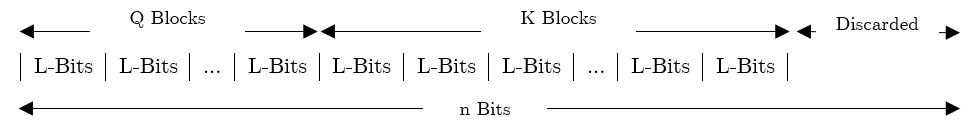
\includegraphics[width=0.8\textwidth]{maurer_ts1.JPG}
        \centering
        \caption{Partitioning for Maurer's Universal Test}
        \label{fig:uts1_part}
    \end{figure}
    
    If $\varepsilon=01011010011101010111$, is considered for an instance, then $n=20$. For $L=2$ and $Q=4$, $K=\floor{\dfrac{n}{L}}-Q=\floor{\dfrac{20}{2}}-4=6$. That would make the initialisation segment $01011010$ and the test segment $011101010111$. $L$-bit blocks could be obtained as follows (Table \ref{tab:ust_segs}).
    
    \begin{table}[h!]
        \centering
        \begin{tabular}{|c|c|c|}
            \hline
            \textbf{Block} & \textbf{Type} & \textbf{Content} \\ \hline
            \textbf{1} & \multirow{4}{*}{\begin{tabular}[c]{@{}c@{}}Initialisation\\ Segment\end{tabular}} & 01 \\ \cline{1-1} \cline{3-3} 
            \textbf{2} &  & 01 \\ \cline{1-1} \cline{3-3} 
            \textbf{3} &  & 10 \\ \cline{1-1} \cline{3-3} 
            \textbf{4} &  & 10 \\ \hline
            \textbf{5} & \multirow{6}{*}{Test Segment} & 01 \\ \cline{1-1} \cline{3-3} 
            \textbf{6} &  & 11 \\ \cline{1-1} \cline{3-3} 
            \textbf{7} &  & 01 \\ \cline{1-1} \cline{3-3} 
            \textbf{8} &  & 01 \\ \cline{1-1} \cline{3-3} 
            \textbf{9} &  & 01 \\ \cline{1-1} \cline{3-3} 
            \textbf{10} &  & 11 \\ \hline
        \end{tabular}
        \caption{Segments of $\varepsilon=01011010011101010111$ for $L=2$ and $@=4$}
        \label{tab:ust_segs}
    \end{table}
    
    \item A table for each possible $L$-bit value is created using the initialisation segment. Here, each $L$-bit combination would be a column in the table ($T_j$ where $j$ is the decimal representation of the combination). Then the block number of the last occurrence of each $L$-bit block is noted in the corresponding column in the table (e.g. \ref{tab:ust_block_pos}). For an instance,
    
    \begin{table}[h!]
        \centering
        \begin{tabular}{|c|c|c|c|c|}
            \hline
            \multirow{2}{*}{} & \multicolumn{4}{c|}{\textbf{$L$-bit Combinations}} \\ \cline{2-5} 
             & 00 & 01 & 10 & 11 \\ \hline
            \textbf{Initialisation} & 0 & 2 & 4 & 0 \\ \hline
        \end{tabular}
        \caption{Block positions of the last occurrences of $L$-bit blocks in the Test Segment}
        \label{tab:ust_block_pos}
    \end{table}
    
    \item Examine each block in the test segment and determine the number of blocks since the last occurrence of that $L$-bit block (i.e. for $i$ where $i$ is the position of the current block in the test segment, $i–T_j$). Replace the value in the table with the location of the current block (i.e. $T_j=i$). Add the calculated distance between re-occurrences of the same $L$-bit block to an accumulating $log_2$ sum of all the differences detected in the $K$ blocks (i.e. $sum=sum+log_2(i–T_j)$). For instance, the cumulative sum for above example could be developed as follows:
    
    \begin{itemize}
        \item For block 5 (the $1^{st}$ test block): 5 is “$01$” hence $T_1$ is increased by 1, and $sum=log_2(5-2) = 1.584962501$.
        \item For block 6: 6 is “$11$” hence $T_3$ is increased by 1, and $sum=1.584962501+log_2(6-0)=1.584962501+2.584962501=4.169925002$.
        \item For block 7: 7 is “$01$” hence $T_1$ is increased by 1, and $sum=4.169925002+log_2(7-5)=4.169925002+1=5.169925002$.
        \item For block 8: 8 is “$01$” hence $T_1$ is increased by 1, and $sum=5.169925002+log_2(8-7)=5.169925002+0=5.169925002$.
        \item For block 9: 9 is “$01$” hence $T_1$ is increased by 1, and $sum=5.169925002+log_2(9-8)=5.169925002+0=5.169925002$.
        \item For block 10: 10 is “$11$” hence $T_3$ is increased by 1, and $sum=5.169925002+log_2(10-6)=5.169925002+2=7.169925002$. 
    \end{itemize}
    
    Once the accumulation is complete, the status of the table that indicates the last occurrences could be as follows (Table \ref{tab:ust_block_pos_final}).
    
    \begin{table}[h!]
        \centering
        \begin{tabular}{|c|c|c|c|c|}
            \hline
            \multirow{2}{*}{} & \multicolumn{4}{c|}{\textbf{$L$-bit Combinations}} \\ \cline{2-5} 
             & 00 & 01 & 10 & 11 \\ \hline
            \textbf{Initialisation} & 0 & 2 & 4 & 0 \\ \hline
            \textbf{5} & 0 & 2 & 4 & 0 \\ \hline
            \textbf{6} & 0 & 5 & 4 & 6 \\ \hline
            \textbf{7} & 0 & 7 & 4 & 6 \\ \hline
            \textbf{8} & 0 & 8 & 4 & 6 \\ \hline
            \textbf{9} & 0 & 9 & 4 & 6 \\ \hline
            \textbf{10} & 0 & 9 & 4 & 10 \\ \hline
        \end{tabular}
        \caption{Final state of the block positions of the last occurrences of $L$-bit blocks in the Test Segment}
        \label{tab:ust_block_pos_final}
    \end{table}
    
    \item Compute the test statistic $f_n=\dfrac{1}{K}\sum_{i=Q+1}^{Q+K}log_2(i-T_j)$, where $T_j$ is the label of the column corresponding to the decimal representation of the contents of the $i^{\text{th}}$ $L$-bit block. For the above case $f_n=\dfrac{7.169925002}{6}=1.1949875$.
    
    \item Compute the $P$-value given by $\text{erfc}\bigg(\abs*{\dfrac{f_n-\text{expectedValue}(L)}{\sqrt{2}\sigma}}\bigg)$. For $\text{expectedValue}(L)$ and $\sigma$, value combinations are precomputed as tabulated below (Table \ref{tab:ust_exval_var}). Under an assumption of randomness, the sample mean $\text{expectedValue}(L)$ is the theoretical expected value of the computed statistic for given $L$-bit length. The theoretical standard deviation $\sigma$ is given by $c\sqrt{\dfrac{\text{variance}(L)}{K}}$ where $c=0.7-\dfrac{0.8}{L}\bigg(4+\dfrac{32}{L}\bigg)\dfrac{K^{-3/L}}{15}$.
    
    \begin{table}[h!]
        \centering
        \begin{tabular}{|c|c|c|}
            \hline
            \textbf{L} & \textbf{\textit{expectedValue}} & \textbf{\textit{variance}} \\ \hline
            \textbf{6} & 5.2177052 & 2.954 \\ \hline
            \textbf{7} & 6.1962507 & 3.125 \\ \hline
            \textbf{8} & 7.1836656 & 3.238 \\ \hline
            \textbf{9} & 8.1764248 & 3.311 \\ \hline
            \textbf{10} & 9.1723243 & 3.356 \\ \hline
            \textbf{11} & 10.170032 & 3.384 \\ \hline
            \textbf{12} & 11.168765 & 3.401 \\ \hline
            \textbf{13} & 12.168070 & 3.410 \\ \hline
            \textbf{14} & 13.167693 & 3.416 \\ \hline
            \textbf{15} & 14.167488 & 3.419 \\ \hline
            \textbf{16} & 15.167379 & 3.421 \\ \hline
        \end{tabular}
        \caption{\textit{expectedValue}, \textit{variance} combinations for values of $L$}
        \label{tab:ust_exval_var}
    \end{table}
\end{enumerate}

For $f_n$ that significantly differs from the theoretical expected values for $\sigma$ computed above indicates that the sequence is significantly compressible without loosing the information. Such values for $f_n$ would yield $P$-values which are $\leq0.01$ which would be deemed non random. The test requires long sequences of bits ($n\geq(Q+K)L$ for $6\leq L \leq16$, $Q=10\cdot2^L$ and $K=\ceil*{\dfrac{n}{L}-Q}\approx1000\cdot2^L$). Optimum value combinations for $L,Q$ and $n$ are as follows (Table \ref{tab:ust_rec_vals}).

\begin{table}[h!]
    \centering
    \begin{tabular}{|l|c|c|}
        \hline
        \multicolumn{1}{|c|}{\textbf{n}} & \textbf{L} & \textbf{Q} \\ \hline
        $\geq387840$ & 6 & 640 \\ \hline
        $\geq904960$ & 7 & 1280 \\ \hline
        $\geq268480$ & 8 & 2560 \\ \hline
        $\geq4654080$ & 9 & 5120 \\ \hline
        $\geq10342400$ & 10 & 10240 \\ \hline
        $\geq22753280$ & 11 & 20480 \\ \hline
        $\geq49643520$ & 12 & 40960 \\ \hline
        $\geq107560960$ & 13 & 818920 \\ \hline
        $\geq231669760$ & 14 & 163840 \\ \hline
        $\geq496435200$ & 15 & 327680 \\ \hline
        $\geq1059061760$ & 16 & 655360 \\ \hline
    \end{tabular}
    \caption{Recommended value combinations for $L,Q$ and $n$}
    \label{tab:ust_rec_vals}
\end{table}

\subsection{Linear Complexity Test}

This test uses linear complexity to test for randomness. The test determines whether or not the sequence being considered is complex enough to be deemed random. The concept of linear complexity is related to a well known part of most of the key stream generators which is, \acrfull{lfsr} of length $L$ consists of $L$ delay elements each having one input and one output. If the initial state of LFSR is ($\varepsilon_{L-1}, \ldots, \varepsilon_1, \varepsilon_0$), then the output sequence, ($\varepsilon_L, \varepsilon_{L+1}, \ldots$), satisfies the following recurrent formula for $j \geq L$

\[
    \varepsilon_j=(c_1\varepsilon_{j-1}+c_2\varepsilon_{j-2}+\ldots+c_L\varepsilon_{j-L}) \pmod{2}
\]
 
 $c_1,\ldots,c_L$ are the coefficients of the connection polynomial corresponding to a given LFSR. An LFSR is considered to generate a binary sequence if this sequence is the output of the LFSR for some initial state.
 
 \subsubsection{Implementation}

Test execution requires a function $linearComplexity(M,n)$ with the parameters

\begin{itemize}
    \item $M$ - Length of each block
    \item $n$ - Length of the bit string
\end{itemize}

Apart from these, the function should have access to $\varepsilon$ which is the bit string generated by the RNG being tested, and $K$ which is the degrees of freedom as internal parameters. For the tests here, $K=6$ is hard coded. The test execution would generate the statistic $\chi^2(\text{obs})$ which is a measure of how well the observed number of occurrences of fixed length LFSRs matches the expected number of occurrences under an assumption of randomness and which refers to the $\chi^2)$ distribution. Test routine is as enumerated below.

\begin{enumerate}
    \item Partition the string into $N$ blocks, each of $M$-bit long.
    
    \item Using the Berlekamp-Massey algorithm, determine the linear complexity $L_i$ of each block. $L_i$ is the length of the shortest LFSR sequence that generates all bits in the block being tested. Within any $L_i$-bit sequence some combination of the bits, when added together modulo 2 produces the next bit ($L_i+1$) of the sequence \cite{rep_nist_sp_80022}.
    
    For an instance if $\varepsilon=1101011110001$ is considered, then $M=13$, $L_i=4$ and the sequence is produced by adding the \nth{1} and \nth{2} bits within a 4-bit sub sequence to produce the \nth{5}. The examination procedure could be tabulated as follows (Table \ref{tab:lct_s2}).
    
    \begin{table}[]
        \centering
        \begin{tabular}{|l|c|c|c|c|c|}
            \hline
             & \textbf{Bit 1} & \textbf{Bit 2} & \textbf{Bit 3} & \textbf{Bit 4} & \textbf{Bit 5} \\ \hline
            \nth{1} four bits and resulting \nth{5} bit & 1 & 1 & 0 & 1 & 0 \\ \hline
            Bits 2-5 and resulting \nth{6} bit & 1 & 0 & 1 & 0 & 1 \\ \hline
            Bits 3-6 and resulting \nth{7} bit & 0 & 1 & 0 & 1 & 1 \\ \hline
            Bits 4-7 and resulting \nth{8} bit & 1 & 0 & 1 & 1 & 1 \\ \hline
            Bits 5-8 and resulting \nth{9} bit & 0 & 1 & 1 & 1 & 1 \\ \hline
            Bits 6-9 and resulting \nth{10} bit & 1 & 1 & 1 & 1 & 0 \\ \hline
            Bits 7-10 and resulting \nth{11} bit & 1 & 1 & 1 & 0 & 0 \\ \hline
            Bits 8-11 and resulting \nth{12} bit & 1 & 1 & 0 & 0 & 0 \\ \hline
            Bits 9-12 and resulting \nth{13} bit & 1 & 0 & 0 & 0 & 1 \\ \hline
        \end{tabular}
        \caption{Examination result of $\varepsilon=1101011110001$ and $L_i$=4}
        \label{tab:lct_s2}
    \end{table}
    
    For this block, the trial feedback algorithm works. If this were not the case, other feedback algorithms would be attempted for the block (e.g. adding bits 1 and 3 to produce bit 5, or adding bits 1, 2 and 3 to produce bit 6, and so forth).
    
    \item Under an assumption of randomness, calculate the theoretical mean $\mu$ given by
    
    \[
        \mu=\dfrac{M}{2}+\dfrac{(9+(-1)^{M+1})}{36}-\dfrac{(\dfrac{M}{3}+\dfrac{2}{9})}{2^M}
    \]
    
    \item For each substring compute $T_i$ given by $(-1)^M\cdot(L_i-\mu)+\dfrac{2}{9})$
    
    \item Record the $T_i$ values in $\nu_0,\ldots,\nu_6$ as follows (Table \ref{tab:lct_s3}).
    
    \begin{table}[h!]
        \centering
        \begin{tabular}{|l|c|}
            \hline
            \multicolumn{1}{|c|}{\textbf{Condition}} & \textbf{Increment} \\ \hline
            $T_i\leq-2.5$ & $\nu_0++$ \\ \hline
            $-2.5<T_i\leq-1.5$ & $\nu_1++$ \\ \hline
            $-1.5<T_i\leq-0.5$ & $\nu_2++$ \\ \hline
            $-0.5<T_i\leq0.5$ & $\nu_3++$ \\ \hline
            $0.5<T_i\leq1.5$ & $\nu_4++$ \\ \hline
            $1.5<T_i\leq2.5$ & $\nu_5++$ \\ \hline
            $T_i>2.5$ & $\nu_6++$ \\ \hline
        \end{tabular}
        \caption{$T_i$ values and corresponding increment positions}
        \label{tab:lct_s3}
    \end{table}
    
    \item Compute $\chi^2(\text{obs}) = \sum_{i=0}^{K}\dfrac{(\nu_i-N\pi_i)^2}{N\pi_i}$, for $\pi_1=0.010417$, $\pi_2=0.03125$, $\pi_3=0.125$, $\pi_4=0.25$, $\pi_1=0.0625$ and $\pi_6=0.020833$, which are precomputed based on the mathematical model for this test.
    
    \item Compute the $P$-value which is given bu $\text{igamc}(\dfrac{K}{2}, \dfrac{\chi^2(\text{obs})}{2})$
\end{enumerate}

$P$-values which are $<0.01$ indicate that the observed frequency counts of $T_i$ stored in the $\nu_i$ bins varies from the expected values. The distribution of the frequency of the $T_i$ stored in the $\nu_i$ bins should be proportional to the computed $\pi_i$. Inputs sizes are recommended to be chosen such that $n\geq10^6$, $500 \leq M \leq 5000$ and $N\geq200$ for the $\chi_2$ result to be valid.

\subsection{Serial Test}

This test accounts the frequency of all possible overlapping $m$-bit patterns across the whole sequence. This test aims at determining whether the number of occurrences of the $2^m$ $m$-bit overlapping patterns is approximately the same as that would be expected for a random sequence. Random sequences are expected to demonstrate uniformity. That is, every $m$-bit pattern has the similar probability of appearing as every other $m$-bit pattern. Given $m=1$, this is equivalent to the frequency test discussed in subsection \ref{subsec:monobits}.

\subsubsection{Implementation}

Test execution requires a function $serial(m,n)$ with the parameters

\begin{itemize}
    \item $m$ - Length of each block
    \item $n$ - Length of the bit string
\end{itemize}

Apart from these, the function should have access to $\varepsilon$ which is the bit string generated by the RNG being tested. The test execution would generate the statistic $\bigtriangledown\psi^2_m(\text{obs})$ and $\bigtriangledown\psi^2_m(\text{obs})$ which are measures of how well the observed observed frequencies of $m$-bit patterns match the expected frequencies of $m$-bit patterns, which refer to the $\chi^2)$ distribution. Test routine is as enumerated below.

\begin{enumerate}
    \item Augment the test sequence by appending the first $m-1$ bits of the sequence to the end of it. For an instance for the bit string $\varepsilon=0011011101$ where $n=10$, if $m=3$ $\varepsilon'=001101110100$, if $m=2$ $\varepsilon'=00110111010$, if $m=1$ $\varepsilon'=0011011101$ and so forth.
    
    \item Determine the frequencies for all $m$-bit blocks, $m-1$-bit blocks and $m-2$-bit blocks. given that $\nu_{i_1 \ldots i_m}$ denotes the frequency of $i_1 \ldots i_m$ bit pattern, $\nu_{i_1 \ldots i_{m-1}}$ denotes the frequency of $i_1 \ldots i_{m-1}$ bit pattern and $\nu_{i_1 \ldots i_{m-2}}$ denotes the frequency of $i_1 \ldots i_{m-2}$ bit pattern.
    
    For the instance above where $m=3$, the frequencies of all 3-bit blocks are given by $\nu_{000}=0$, $\nu_{001}=1$, $\nu_{010}=1$, $\nu_{011}=2$, $\nu_{100}=1$, $\nu_{101}=2$, $\nu_{110}=2$ and $\nu_{111}=0$. The frequencies of all 2-bit blocks are given by $\nu_{00}=1$, $\nu_{01}=3$, $\nu_{01}=3$, and $\nu_{11}=3$. The frequencies of all 1-bit blocks are given by $\nu_{0}=4$ and $\nu_{1}=6$.
    
    \item Compute $\psi^2_x=\dfrac{2^x}{n}\sum_{i_1 \ldots i_x} \bigg( \nu_{i_1 \ldots i_x} - \dfrac{n}{2^x} \bigg) ^2 = \dfrac{2^x}{n}\sum_{i_1 \ldots i_x}\nu^2_{i_1 \ldots i_x} - n$ for $x \in \{m, m-1, m-2\}$. For the instance above $\psi^2_3=2.8$, $\psi^2_2=1.2$ and $\psi^2_1=0.4$.
    
    \item Compute $\bigtriangledown\psi^2_m=\psi^2_m-\psi^2_{m-1}$ and $\bigtriangledown^2\psi^2_m=\psi^2_m-2\psi^2_{m-1}+\psi^2_{m-2}$.
    
    \item Compute $P$-value 1 given by $\text{igamc}(2^{m-2}, \bigtriangledown\psi^2_m)$ and $P$-value 2 given by $\text{igamc}(2^{m-3}, \bigtriangledown^2\psi^2_m)$.
\end{enumerate}

Either one of $\bigtriangledown\psi^2_m$ or $\bigtriangledown^2\psi^2_m$ being quite large, implies that the $m$-bit block is lacks in uniformity expected, which would cause $P$-values $<0.01$ yielding the bit string to be non random. It is recommended to choose $m$ and $n$ such that $m < \floor*{log_2n}-2$.

\subsection{Approximate Entropy Test}

This test also focuses on the frequency of all possible overlapping $m$-bit patterns across the whole sequence. During the test, the frequency of overlapping blocks of two adjacent/consecutive lengths (e.g. $m$ and $m+1$) are compared against the expected result for a random sequence. 

\subsubsection{Implementation}

Test execution requires a function $approximateEntropy(m,n)$ with the parameters

\begin{itemize}
    \item $m$ - Length of each block - In this case the length of the first block used in the test.
    \item $n$ - Length of the bit string
\end{itemize}

Apart from these, the function should have access to $\varepsilon$ which is the bit string generated by the RNG being tested. The test execution would generate the statistic $\chi^2(\text{obs})$ which is a measure of how well the observed value of $\text{ApEn}(m)$ (refer to step 6 in the enumeration of test routine) matches the expected value, which refer to the $\chi^2)$ distribution. Test routine is as enumerated below.

\begin{enumerate}
    \item Augment the test sequence by appending the first $m-1$ bits of the sequence to the end of it. For an instance for the bit string $\varepsilon=0011011101$ where $n=10$, if $m=3$ $\varepsilon'=001101110100$, if $m=2$ $\varepsilon'=00110111010$, if $m=1$ $\varepsilon'=0011011101$ and so forth. Let the length of the augmented bit string be given by $n'$.
    
    \item Count the frequencies of each $m$-bit combination $i$ by considering a sliding window of $\varepsilon_{j, \ldots, m-1}$ length on the augmented bit string $\varepsilon'$ for $0 \leq j \leq n'$. For the instance above where $m=3$, 3-bit overlapping blocks are the set $\{010, 100, 001, 011, 110, 101, 010, 101, 010, 101\}$. The counts for each $i$ would be $\#000=0$, $\#001=1$, $\#010=3$, $\#011=1$, $\#100=1$, $\#101=3$, $\#110=1$ and $\#111=0$.
    
    \item Compute $C^m_i=\dfrac{i}{n}$ for each decimal value of $i$. For the instance above $C^3_000=0$, $C^3_001=0.1$, $C^3_010=0.3$, $C^3_011=0.1$, $C^3_100=0.1$, $C^3_101=0.3$, $C^3_110=0.1$ and $C^3_111=0$.
    
    \item Compute $\gamma^m=\sum^{2^m-1}_{i=0}\pi_ilog\pi_i$, where $\pi_i=C^m_j$ and $j=log_2i$.
    
    \item Repeat the steps 1-4 for $m+1$.
    
    \item Compute the test statistic $\chi^2=2n(log2-\text{ApEn(m)})$, where $\text{ApEn(m)}=\gamma^m-\gamma^{m-1}$.
    
    \item Compute the $P$-value given by $\text{igamc}\bigg(2^{m-1},\dfrac{\chi^2}{2}\bigg)$.
\end{enumerate}

Small values of \textit{ApEn(m)} would imply strong regularity in the bit string while large values would imply substantial fluctuation or irregularity. It is recommended to choose $m$ and $n$ in such a way that $m < \floor*{log_2n}-5$.

\subsection{Cumulative Sum Test}

The test is based on the maximum absolute value of the partial sums of the sequence $\varepsilon$ where $\varepsilon_i=\pm1$. This cumulative sum could be comprehended as a random walk. For a sequence to be deemed random, the excursions of the random walk should lie close to zero. For certain types of non-random sequences, the excursions of this random walk from zero will be large. Large values of this statistic indicate that the sequence has a too large number of 1's or 0's at the \textit{wings} (either end of the sequence is called \textit{wings}) of the sequence. Small values indicate that the intermixing of the 1's and 0's are too even for the sequence given.

\subsubsection{Implementation}

Test execution requires a function $cumulativeSums(mode,n)$ with the parameters

\begin{itemize}
    \item $mode$ - A switch that indicates the direction of the test.
    \item $n$ - Length of the bit string
\end{itemize}

Apart from these, the function should have access to $\varepsilon$ which is the bit string generated by the RNG being tested. The test execution would generate the statistic $z$ which is the largest excursion from the origin of the cumulative sums in the corresponding ($-1$, $+1$), which refer to the $\chi^2)$ distribution. Test routine is as enumerated below.

\begin{enumerate}
    \item Obtain the normalised sequence $X$ from the input sequence $\varepsilon$ by replacing each bit $\varepsilon_i$ of the string with $X_i$ where $X_i=2\varepsilon_i-1$. For an instance $\varepsilon=1011010111$, $X=1, (-1), 1, 1, (-1), 1, (-1), 1, 1, 1$.
    
    \item Compute the partial sums $S_k=\sum_{i=1}^{k}X_i$ for $\{k\lvertk\in\mathbb{Z}\land 1 \leq k \leq 10\}$. For backward mode (i.e. $mode=1$) $S_k=\sum_{i=k}^{n-k+1}X_i$ for $\{k\lvertk\in\mathbb{Z}\land 1 \leq k \leq 10\}$.
    
    For the instance above, when $mode=0$
    
    \hfill\begin{minipage}{\dimexpr\textwidth-3cm}
    	$S_{1} = 1$
    	
    	$S_{2} = 1 + (-1) = 0$
    	
    	$S_{3} = 1 + (-1) + 1 = 1$
    	
    	$S_{4} = 1 + (-1) + 1 + 1 = 2$
    	
    	$S_{5} = 1 + (-1) + 1 + 1 + (-1) = 1$
    	
    	$S_{6} = 1 + (-1) + 1 + 1 + (-1) + 1 = 2$
    	
    	$S_{7} = 1 + (-1) + 1 + 1 + (-1) + 1 + (-1) = 1$
    	
    	$S_{8} = 1 + (-1) + 1 + 1 + (-1) + 1 + (-1) + 1 = 2$
    	
    	$S_{9} = 1 + (-1) + 1 + 1 + (-1) + 1 + (-1) + 1 + 1 = 3$
    	
    	$S_{10} = 1 + (-1) + 1 + 1 + (-1) + 1 + (-1) + 1 + 1 + 1 = 4$
    \xdef\tpd{\the\prevdepth}
    \end{minipage}
    
    \item Find $z=max(S_k)$ which is the largest of the absolute values of the partial sums. For the instance above $z=4$.
    
    \item Compute the $P$-value given by $1 - A + B$ where
    
    \[
        A = \sum_{k=\dfrac{\dfrac{-n}{z}+1}{4}}^{\dfrac{\dfrac{n}{z}-1}{4}}\Bigg[\Phi\Bigg(\dfrac{(4k+1)z}{\sqrt{n}}\Bigg) - \Phi\Bigg(\dfrac{(4k-1)z}{\sqrt{n}}\Bigg)\Bigg]
    \]
    and
    \[
        B = \sum_{k=\dfrac{\dfrac{-n}{z}-3}{4}}^{\dfrac{\dfrac{n}{z}-1}{4}}\Bigg[\Phi\Bigg(\dfrac{(4k+3)z}{\sqrt{n}}\Bigg) - \Phi\Bigg(\dfrac{(4k+1)z}{\sqrt{n}}\Bigg)\Bigg]
    \]
    
    where $\Phi$ is the Standard Normal Cumulative Probability Distribution function.
\end{enumerate}

For $mode=0$, bit string which tend to have large number of 1's or 0's at the early stages would have large values for the text statistic. For $mode=1$, bit string which tend to have large number of 1's or 0's at the latter stages would have large values for the text statistic. When the intermixing of 1's and 0's are too even, the test statistic would indicate smaller values. Recommended input size (i.e. the value of $n$) should be such that $n \geq 100$ \cite{rep_nist_sp_80022}.

\subsection{Random Excursions Test}

This test is based on the number of cycles having exactly K visits in a cumulative sum random walk. Initially the sequence $\varepsilon$ is transformed so that for any $i\in\mathbb{Z}^+$ $\varepsilon_1=\pm1$ and then the cumulative sum random walk is derived. A \textit{cycle in a random walk} is a segment of consecutive cumulative sums, which the both sum values at the beginning and the end are zero. (e.g. for $S=\{1,2,0,-1,-3,0,2,3,0\}$, both $0,-1,-3,0$ and $0,2,3,0$ are cycles in the random walk). The test intends to determine if the number of visits to a particular state within a cycle deviates from what one would expect for a random sequence. This test is actually a series of eight tests (and conclusions), one test and conclusion for each of the states: $-4, -3, -2, -1$ and $+1, +2, +3, +4$.

\subsubsection{Implementation}

Test execution requires a function $cumulativeSums(mode,n)$ with the parameters

\begin{itemize}
    \item $n$ - Length of the bit string
\end{itemize}

Apart from these, the function should have access to $\varepsilon$ which is the bit string generated by the RNG being tested. The test execution would generate the statistic $\chi^2(\text{obs})$ which is the degree of similarity between the observer number of state visits and the expected number of state visits within a cycle match, which refer to the $\chi^2)$ distribution. Test routine is as enumerated below.

\begin{enumerate}
    \item Obtain the normalised sequence $X$ from the input sequence $\varepsilon$ by replacing each bit $\varepsilon_i$ of the string with $X_i$ where $X_i=2\varepsilon_i-1$. For an instance $\varepsilon=0110110101$, $X=(-1), 1, 1, (-1), 1, 1, (-1), 1, (-1), 1$.
    
    \item Compute the partial sums $S_k=\sum_{i=1}^{k}X_i$ for $\{k\lvert k \in \mathbb{Z}\land 1 \leq k \leq 10\}$.
    
    For the instance above
    
    \begin{table}[h!]
        \centering
        \begin{tabular}{ll}
            $S_1=-1$ & $S_6=2$ \\
            $S_2=0$ & $S_7=1$ \\
            $S_3=1$ & $S_8=2$ \\
            $S_4=0$ & $S_9=1$ \\
            $S_5=1$ & $S_{10}=2$
        \end{tabular}
    \end{table}
    
    The sequence of sums are given by $S=[-1, 0, 1, 0, 1, 2, 1, 2, 1, 2]$.
    
    \item Augment $S$ and obtain $S'$ by adding zero at the beginning and the end of the sequence. For the above instance $S'=[0, -1, 0, 1, 0, 1, 2, 1, 2, 1, 2, 0]$. The random walk could be graphically depicted as below (Figure \ref{fig:ret1_walks}).
    
    \begin{figure}[h!]
        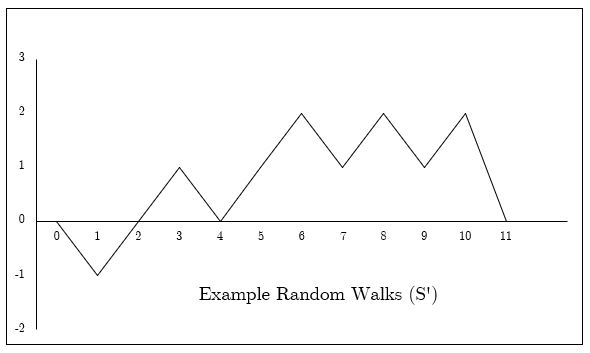
\includegraphics[width=0.8\textwidth]{rand_walks.JPG}
        \centering
        \caption{Example Random Walks ($S'$)}
        \label{fig:ret1_walks}
    \end{figure}
    
    \item Determine $J$ where $J$ is the number of cycles in the sequence. If $J<500$ the test shall be discontinued as $J\times\pi_i$ (where $\pi_i$ is the minimum probability which is predetermined as tabulated in NIST SP 800-22 (Page 3-24))\cite{rep_nist_sp_80022} must be $\geq5$ in order to satisfy the empirical rule for $\chi^2$ computations. For the instance above, $J=3$ and the cycles would be $[0, -1, 0]$, $[0, 1, 0]$ and $[0, 1, 2, 1, 2, 1, 2, 0]$ respectively.
    
    \item For each of the cycles, count the frequency of $x$ within the cycle for $\{x\lvert x \in \mathbb{Z}\land -4 \leq k \leq 4 \land x \neq 0\}$. For the example above, the frequencies could be tabulated as follows (Table \ref{table:ret1_freq}).
    
    \begin{table}[h!]
        \centering
        \begin{tabular}{|c|c|c|c|}
            \hline
            \multirow{2}{*}{\textbf{\begin{tabular}[c]{@{}c@{}}State\\ \textit{x}\end{tabular}}} & \multicolumn{3}{c|}{\textbf{Cycles}} \\ \cline{2-4} 
             & \textbf{\begin{tabular}[c]{@{}c@{}}Cycle 1\\ (0,-1,0)\end{tabular}} & \textbf{\begin{tabular}[c]{@{}c@{}}Cycle 2\\ (0,1,0)\end{tabular}} & \textbf{\begin{tabular}[c]{@{}c@{}}Cycle 3\\ (0,1,2,1,2,1,2,0)\end{tabular}} \\ \hline
            \textbf{-4} & 0 & 0 & 0 \\ \hline
            \textbf{-3} & 0 & 0 & 0 \\ \hline
            \textbf{-2} & 0 & 0 & 0 \\ \hline
            \textbf{-1} & 1 & 0 & 0 \\ \hline
            \textbf{1} & 0 & 1 & 3 \\ \hline
            \textbf{2} & 0 & 0 & 3 \\ \hline
            \textbf{3} & 0 & 0 & 0 \\ \hline
            \textbf{4} & 0 & 0 & 0 \\ \hline
        \end{tabular}
        \caption{Frequency Tabulation for occurrences of $x$}
        \label{table:ret1_freq}
    \end{table}
    
    \item For each state $x$, count $\nu_k(x)$ which is the total number of cycles in which state $x$ occurs exactly $k$ times from among all the cycles for $\{\k \lvert k \in \overline{\mathbb{Z}} \land k \leq 5\}$. For all $k \geq 5$, the count is stored in the column for $k=5$. For the instance above, these statistics could be tabulated as follows (Table \ref{tab:ret2_cyc_ct}).
    
    \begin{table}[h!]
        \centering
        \begin{tabular}{|c|c|c|c|c|c|c|}
            \hline
            \multirow{2}{*}{\textbf{\begin{tabular}[c]{@{}c@{}}State\\ (\textit{x})\end{tabular}}} & \multicolumn{6}{c|}{\textbf{Number of Cycles}} \\ \cline{2-7} 
             & 0 & 1 & 2 & 3 & 4 & 5 \\ \hline
            \textbf{-4} & 3 & 0 & 0 & 0 & 0 & 0 \\ \hline
            \textbf{-3} & 3 & 0 & 0 & 0 & 0 & 0 \\ \hline
            \textbf{-2} & 2 & 1 & 0 & 0 & 0 & 0 \\ \hline
            \textbf{-1} & 2 & 1 & 0 & 0 & 0 & 0 \\ \hline
            \textbf{1} & 1 & 1 & 0 & 1 & 0 & 0 \\ \hline
            \textbf{2} & 2 & 0 & 0 & 1 & 0 & 0 \\ \hline
            \textbf{3} & 3 & 0 & 0 & 0 & 0 & 0 \\ \hline
            \textbf{4} & 3 & 0 & 0 & 0 & 0 & 0 \\ \hline
        \end{tabular}
        \caption{Number of cycles that contains each state $x$}
        \label{tab:ret2_cyc_ct}
    \end{table}
    
    \item For each of the eight states, compute the test statistic $\chi^2(\text{obs})$
    
    \[
        \chi^2(\text{obs})=\sum_{k=0}^{5}\dfrac{(\nu_k(x)-J\pi_k(x))^2}{J\pi_k(x)}
    \]
    
    where $\pi_k(x)$ is the probability that the state $x$ occurs $k$ items in a random distribution. Value of $\pi$ could be calculated using the following equations.
    
    \[
        \pi_0 = 1-\dfrac{1}{2\lvert x \rvert}
    \]
    
    \[
        \pi_k = \dfrac{1}{4x^2}\Bigg(1-\dfrac{1}{2\lvert x \rvert}\Bigg)^{k-1}; \{k \lvert k \in \mathbb{Z}^+ \land k \leq 5\}
    \]
    
    \[
        \pi_5 = \dfrac{1}{2\lvert x \rvert}\Bigg(1-\dfrac{1}{2\lvert x \rvert}\Bigg)^4
    \]
    
    This will generate a $\chi^2(\text{obs})$ for each state $x$.
    
    \item For each state $x$, compute $P$-value with $\text{igamc}\bigg(\dfrac{5}{2},\dfrac{\chi^2(\text{obs})}{2}\bigg)$.
\end{enumerate}

$\chi^2(\text{obs})$ values which are excessively large, indicate that the sequence demonstrates deviation from the theoretical distribution for a given state across all cycles, yielding $P$-values which are $<0.01$. NIST recommends that each string being tested should be at least $10^6$ bits long (i.e. $n\geq10^6$) \cite{rep_nist_sp_80022}.

\subsection{Random Excursion Variant Test}

This test takes the \textit{total number of times that a particular state is visited} in a cumulative sum random walk into account to determine the statistical quality of the randomness. The deviations of the actual number of visits from the expected number of visits at various states of the random walk will be detected with this test. In fact, the test is repeated over 18 times for statuses denoted by $x$ for $\{x \lvert x \in \mathbb{Z} \land -9 \leq x \leq +9 \land x \neq 0\}$.

\subsubsection{Implementation}

Test execution requires a function $randomExcursionVariant(n)$ with the parameters

\begin{itemize}
    \item $n$ - Length of the bit string
\end{itemize}

Apart from these, the function should have access to $\varepsilon$ which is the bit string generated by the RNG being tested. The test execution would generate the statistic $\xi$ which is the total number of times that a given state $x$ is visited during the entire random walk, which refer to the half normal distribution. Given that $\xi$ is a normal distribution, $\lver\xi\rvert$ should be a half normal distribution. Test routine is as enumerated below.

\begin{enumerate}
    \item Obtain the normalised sequence $X$ from the input sequence $\varepsilon$ by replacing each bit $\varepsilon_i$ of the string with $X_i$ where $X_i=2\varepsilon_i-1$. For an instance $\varepsilon=0110110101$, $X=(-1), 1, 1, (-1), 1, 1, (-1), 1, (-1), 1$.
    
    \item Compute the partial sums $S_k=\sum_{i=1}^{k}X_i$ for $\{k\lvert k \in \mathbb{Z}\land 1 \leq k \leq 10\}$.
    
    For the instance above
    
    \begin{table}[h!]
        \centering
        \begin{tabular}{ll}
            $S_1=-1$ & $S_6=2$ \\
            $S_2=0$ & $S_7=1$ \\
            $S_3=1$ & $S_8=2$ \\
            $S_4=0$ & $S_9=1$ \\
            $S_5=1$ & $S_{10}=2$
        \end{tabular}
    \end{table}
    
    The sequence of sums are given by $S=[-1, 0, 1, 0, 1, 2, 1, 2, 1, 2]$.
    
    \item Augment $S$ and obtain $S'$ by adding zero at the beginning and the end of the sequence. For the above instance $S'=[0, -1, 0, 1, 0, 1, 2, 1, 2, 1, 2, 0]$. The random walk could be graphically depicted as below (Figure \ref{fig:revt1_walks}).
    
    \begin{figure}[h!]
        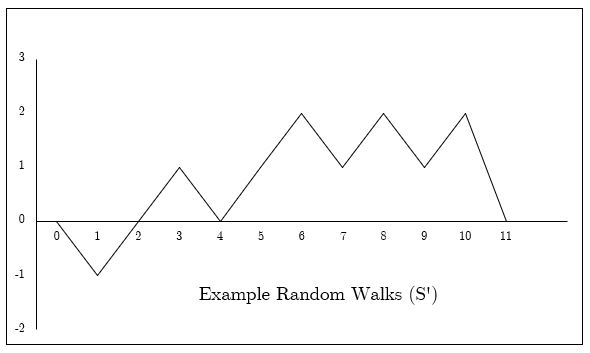
\includegraphics[width=0.8\textwidth]{rand_walks.JPG}
        \centering
        \caption{Example Random Walks ($S'$) (Random Excursion Variant)}
        \label{fig:revt1_walks}
    \end{figure}
    
    \item Count $\xi(x)$ which is the total number of times that each state $x$ is reached during the complete random walk, for all 18 states. For the above instance $\xi(-1)=1$, $\xi(1)=4$, $\xi(2)=3$ and all other $\xi(x)=0$.
    
    \item For each $\xi(x)$, compute the $P$-value given by
    
    \[
        \textit{erfc}=\Bigg(\dfrac{\lvert \xi(x)-J \rvert}{\sqrt{2J(4\lvert x \rvert-2)}}\Bigg)
    \]
    
\end{enumerate}

If the sequence is random, then the test statistic will be about 0. If there are too many 1's or too many 0's, then the test statistic will be large, causing $P$-values which are $<0.01$, yielding the string to be non random. NIST recommends that each string being tested should be at least $10^6$ bits long (i.e. $n\geq10^6$) \cite{rep_nist_sp_80022}.

\section{Common Sources of Bit Strings}

There are a variety of mathematical components such as constants, functions and so forth which are yielding infinite strings of numbers. It all begins at the principles of counting and number theory. There are several different classes of numbers such as integers ($\mathbb{Z}$), real numbers ($\mathbb{R}$), rational ($\mathbb{Q}$) and irrational ($\mathbb{Q}'$) and so forth. All these categorisations are based on how they behave when they are graphically depicted on the \textit{Line of Numbers}. Out of these, rational numbers which are not integers (i.e. ($\mathbb{Q} - \mathbb{Z}$) and irrational numbers ($\mathbb{Q}'$) are quite interesting in terms of \textit{Number Representation in Digital Circuits}. This is because of the properties of binary numbers and their behaviour in different representations. All of the above numbers ($(\mathbb{Q} - \mathbb{Z}) \cup \mathbb{Q}'$) are having fractions of whole numbers (e.g. $1/2$ is also represented as $0.5$ which is a part/fraction of a number). Based on how they behave in decimal number system, they are categorised as follows.

\begin{enumerate}
    \item Terminating Decimals - Numbers that has a finite number of places beyond the decimal point (e.g. $\dfrac{1}{2}$)
    \item Recurring Decimals - Numbers that which its fraction has a whole or part of a finite numbers, which are recurring as a pattern. There could be two different types.
    \begin{enumerate}
        \item The decimal part, called the period, is repeated endlessly (e.g. $3.222...=3.\dot{2}$ and $3.217217...=3.\dot{2}1\dot{7}$)
        \item The period has an irregular part followed by a regular part repeated endlessly (e.g. $0.00522222... = 0.005\dot{2}$ and $4.55127127... = 4.55\dot{1}2\dot{7}$)
    \end{enumerate}
    \item Non terminating/Infinite Decimals - Fractional part is extended infinitely. (e.g. $\pi = 3.141592653\ldots$)
\end{enumerate}

When these numbers are represented in a digital computer, there were several different challenges that which some of them still exist in certain cases. Today, most common representation of decimal numbers, used in modern binary computers is \textit{Floating Point Representations}. However, it is a widely accepted fact that floating point is not an exact representation of a fractional value. In reality, floating point representation is an approximation of the actual fractional value. This result however, yields some interesting results which are identified and meticulously discussed in section \ref{subsec:float_attr}.

In addition to these, enormous amounts of information are being shared in the modern world. Due to the amount of different types of devices, different connectivity technologies available for communication over \acrfull{http} and also the extensive usage of HTTP for business application development has paved the way for an environment which is rich of electronic data. Depending on the different protocols technologies being used, large amounts of metadata which are required to establish, secure, maintain and terminate connectivity between different interfaces are also included in this electronic data rich environment. So, it is fair to conclude that in such an environment there could be certain possible sources which their results/output is random. The existence of such and if available, how useful they are, needs to be taken into account. During this, it is important to focus on the following aspects.

\begin{itemize}
    \item Availability - Whether such data sources are available
    \item Accessibility - Whether accessing such data sources is feasible
    \item Mechanisms for extracting data from such sources
    \item Mechanisms for distillation of such data
    \item Mechanisms for hardening of such data so that they are useful in \textit{security critical applications} such as cryptography
\end{itemize}

\section{Encryption}

Encryption is the process of concealing the true meaning of a message by means of substitution and transposition or some other mathematical means such as \textit{trapdoor functions}. There is a heap of research and literature that could be considered in this aspect. However, the focus on encryption for the scope of this study, is to use it in the process of hardening the generated output to meet the cryptographic security requirements.

\subsection{Advanced Encryption Standard}\label{subsec:aes}

The \acrfull{aes} (also known as \textit{Rijndael}) is a standard for encrypting data communications accepted by the NIST in 2001. AES infact is a refinement of the Rijndael block cipher Vincent Rijmen and Joan Daemen, two Belgian cryptographers. Rijndael encompasses a family of encryption schemes that supports a multitude of block and key sizes. For AES, three members of the Rijndael family were chosen by the NIST, with block lengths of 128, 192 and 256 bits.

AES encryption is four staged process which could be outlined as follows.

\begin{enumerate}
    \item \ilcode{KeyExpansion} — round keys are derived from the cipher key using Rijndael's key schedule. AES requires a separate 128-bit round key block for each round plus one more.
    
    \item Initial round key addition: \ilcode{AddRoundKey} — each byte of the state is combined with a block of the round key using bit wise xor.
    
    \item 9, 11 or 13 rounds for each key length respectively:
    \begin{enumerate}
        \item \ilcode{SubBytes} — a \textbf{\textit{non-linear}} substitution step that replaces each byte based on a lookup table.
        
        \item \ilcode{ShiftRows} — a transposition step where the last three rows of the state shifted to right in a cyclic manner.
        
        \item \ilcode{MixColumns} — a linear mixing operation which operates on the columns of the state, The four bytes of each column are combined here.
        
        \item \ilcode{AddRoundKey}
    \end{enumerate}
    
    \item Final round (giving a total of 10, 12 or 14 rounds for each key size):
    \begin{enumerate}
        \item \ilcode{SubBytes}
        \item \ilcode{ShiftRows}
        \item \ilcode{AddRoundKey}
    \end{enumerate}
\end{enumerate}

\subsection{Block Cipher Modes of Operation}

Block ciphers have various modes of operation, which could be enumerated as follows.

\begin{enumerate}
    \item \acrfull{ecb} - This is the simplest form that a block cipher could be employed in. There, each input block is encrypted in isolation from the previous blocks. Due to this isolation of blocks in operation, certain properties of the plain text such as regions, might be preserved in the cipher text. Hence this is considered to be weak. Yet, this is useful in certain communication channels which are inherently non-reliable, due to the fact that communication errors are not propagated. The process could be graphically depicted as follows (Figure \ref{fig:enc_ecb}).
    
    \begin{figure}[h!]
        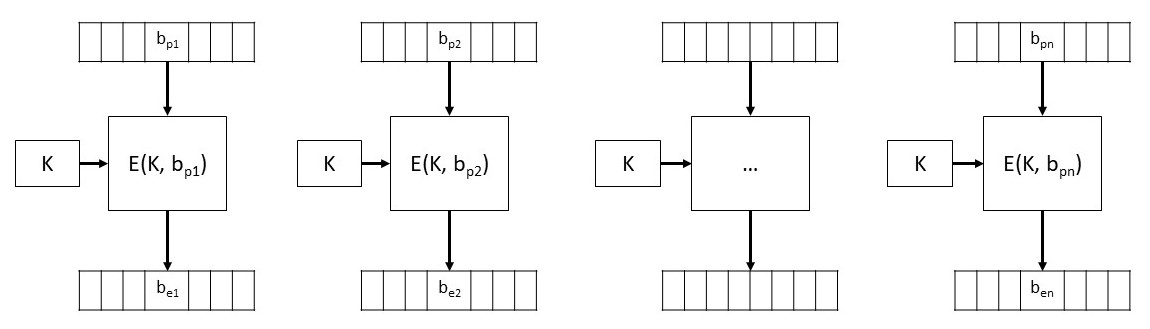
\includegraphics[width=0.8\textwidth]{ecb.JPG}
        \centering
        \caption{\acrfull{ecb} Encryption}
        \label{fig:enc_ecb}
    \end{figure}
    
    \item \acrfull{cbc} - This model introduces an additional step that includes an XOR operation on the plain text block and an IV, that which its output is encrypted with the key. For each successive blocks, the previous block's cipher text becomes the IV. The process could be graphically depicted as follows (Figure \ref{fig:enc_cbc}).
    
    \begin{figure}[h!]
        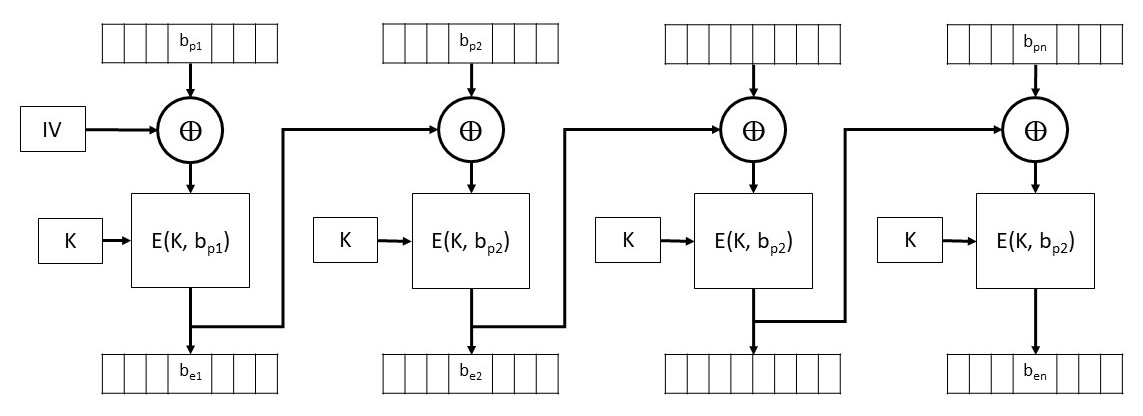
\includegraphics[width=0.8\textwidth]{cbc.JPG}
        \centering
        \caption{\acrfull{cbc} Encryption}
        \label{fig:enc_cbc}
    \end{figure}
    
    Even though this effectively ties each block together, in order to to allow decryption of the message by the recipient, the IV should be shared with the recipient. If an intruder manages to predict the IV, then the encryption would not be resistant to \textit{chosen plain text attacks}\footnote{a cryptanalyst can choose arbitrary plain text data to be encrypted and then he receives the corresponding cipher text}. If the IV is chosen to be some input such as a user password, then it requires to be encrypted using a separate key. IVs should be changed after some time, so as to not to make the system vulnerable to chosen plain text attacks. Also, an isolated error of a single bit during the transmission of the cipher text would be propagated across the rest of the cipher text, yielding the whole cipher text useless. in decryption.
    
    \item \acrfull{cbf} - This mode of operation is quite similar to the CBC, except for that the IV for each iteration/block is encrypted with the key. Then, the resultant is XORed with the plain text block, which will provide the IV for the next iteration. The process could be graphically depicted as follows (Figure \ref{fig:enc_cbf}).
    
    \begin{figure}[h!]
        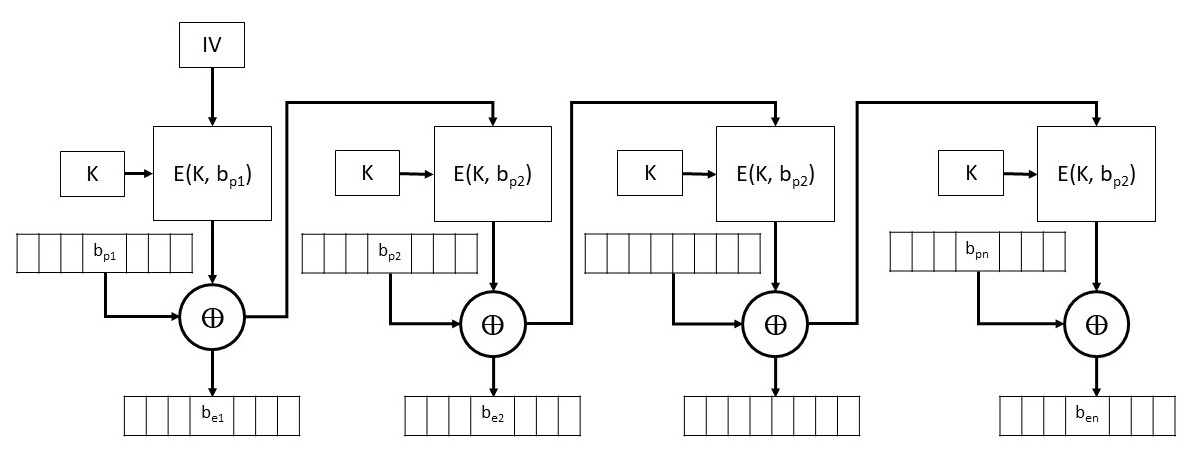
\includegraphics[width=0.8\textwidth]{cbf.JPG}
        \centering
        \caption{\acrfull{cbf} Encryption}
        \label{fig:enc_cbf}
    \end{figure}
    
    This is also vulnerable to error propagation during encryption, due to the tying of blocks using the cipher of each block. 
    
    \item \acrfull{obf} - The IV is repeatedly encrypted to provide the IVs for each successive blocks in this mode. This is also a slight variation of the CBF mode discussed previously. The process could be graphically depicted as follows (Figure \ref{fig:enc_obf}).
    
    \begin{figure}[h!]
        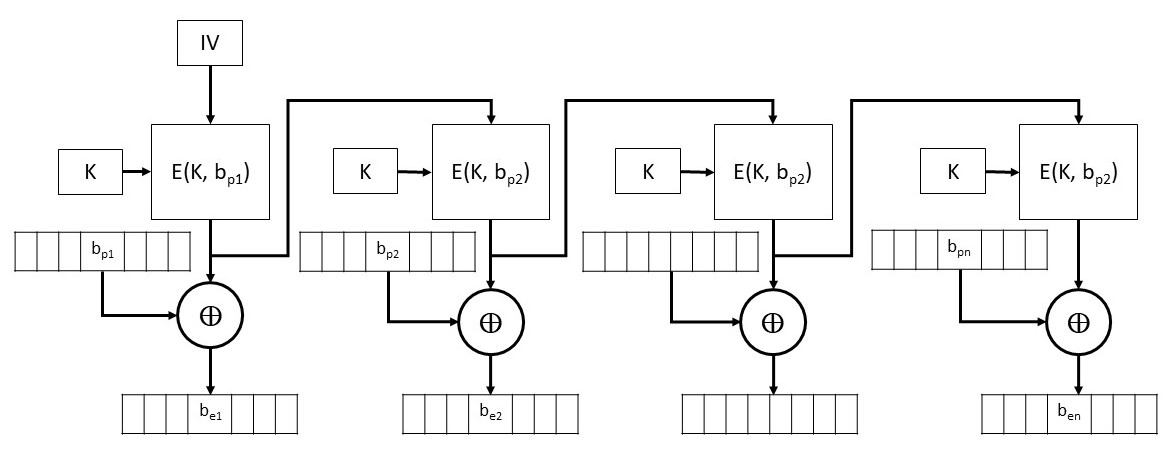
\includegraphics[width=0.8\textwidth]{obf.JPG}
        \centering
        \caption{\acrfull{obf} Encryption}
        \label{fig:enc_obf}
    \end{figure}
    
    If an error occurred in a single bit of plain text or cipher text (for an instance due to a transmission error), only one corresponding cipher text or respectively plain text bit is damaged as well. This could however be recovered using various correction algorithms to restore the previous value of damaged parts of the message. The most critical drawback of OFB is that the state of the system might be repeated due to the repeated encryption of the same plain text. Even though the probability of occurring such situation is quite low, in such a case the plain text blocks will be encrypted with the same corresponding state as previous.
\end{enumerate}

\section{Conceptual Framework}

Based on the knowledge established in the previous sections, the following conceptual framework is formulated to be used in establishment of the scope and further development of the research project (Figure \ref{fig:concept_frame}).

\begin{figure}[h!]
    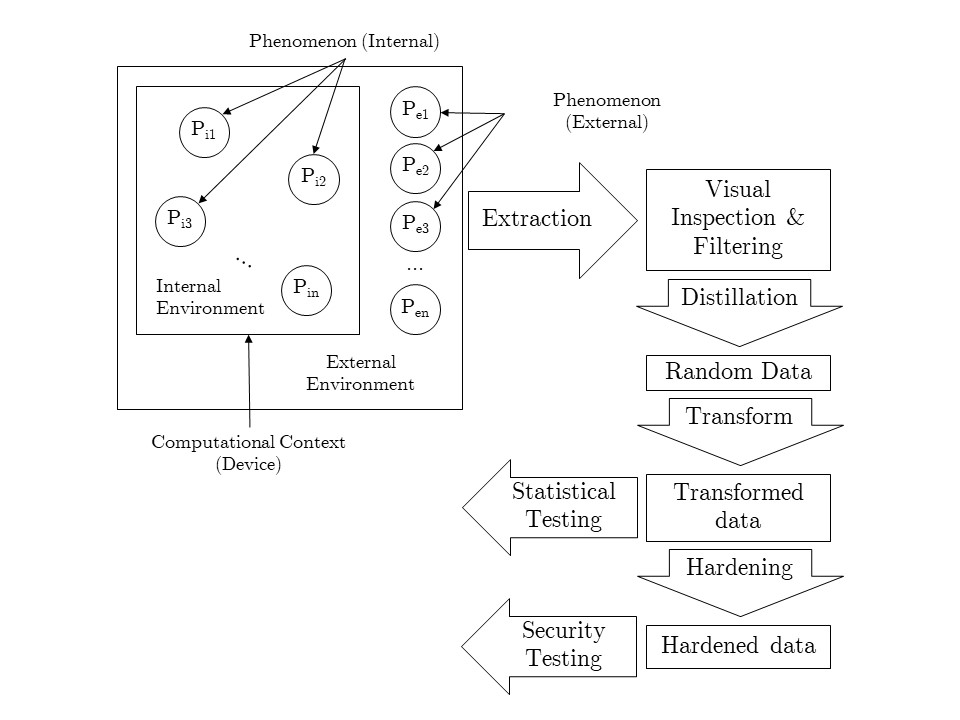
\includegraphics[width=0.8\textwidth]{concept_frame.jpg}
    \centering
    \caption{Conceptual Framework}
    \label{fig:concept_frame}
\end{figure}

\subsection{Elaboration of the Concept}

The research is based on the internal and external phenomena that are observable internally. These sources are monitored and recorded during the \textit{Extraction}. Caution must be exercised when choosing these sources to ensure that an external manipulator has no knowledge or access (ideally) or the least practical knowledge and access. Based on these criteria, the observations recorded are filtered during the \textit{Visual Inspection and Filtering} stage.

The data collected from the filtered sources would undergo a distillation process to extract the exact values and filter them based on the criteria demanded by the transformation work flow, which would play the role of \textit{seeds} which would undergo the \textit{Transformation}, which would magnify the values that has been distilled. These transformed data would be taken into evaluation as inputs to the statistical tests suite. To meet the cryptographic security requirements, the data could optionally be hardened by the hardening strategies identified and assessed in the corresponding section \ref{sec:hardening_details}.